 \pdfobjcompresslevel 0
\documentclass[12pt,a4paper,oneside]{extbook}
\usepackage[utf8]{inputenc}
\usepackage[T1]{fontenc}
\usepackage{titlesec}
\titleformat{\chapter}[display]{\normalfont\huge\bfseries}{\chaptertitlename\ \thechapter}{20pt}{\Huge}
\usepackage{tabularx} 
\usepackage{chngcntr}
\usepackage[table]{xcolor}
\usepackage{fancyvrb,xcolor}
\usepackage{moreverb}
\usepackage[french]{babel}
\usepackage{listings}
\usepackage{glossaries}
\makeglossaries
\usepackage{amsmath}
\usepackage{amssymb}
\usepackage{mathrsfs}
\usepackage{titlesec, blindtext, color}
\usepackage{xcolor}
% Color helper used before list items in chapters
\newcommand{\itemcolor}[1]{\color{#1}}
\usepackage{pifont}
\usepackage{enumitem}
\definecolor{listGreen}{RGB}{34,139,34}
\usepackage[Lenny]{fncychap}
\usepackage{nomencl}
\usepackage{graphicx}
\usepackage{float} % for [H] exact placement of floats
\usepackage[section]{placeins} % prevent floats from crossing section boundaries
\usepackage{multirow}
\usepackage{multicol}
\usepackage{algorithm,algorithmic}
\usepackage{pdfpages}
\usepackage{eqparbox,array}
\usepackage{longtable}
\usepackage{adjustbox}
\usepackage{caption}
\usepackage[left=1in, right=1in, top=1in, bottom=1in, includefoot, headheight=28pt]{geometry}
\usepackage{fancyhdr} % header/footer customization
\newcommand{\fonction}[5]
{
  \begin{array}{lrcl}
    #1:&#2& \rightarrow& #3 \\
    & #4&\mapsto&#5
  \end{array}
}

\newtheorem{theo}{\textbf{Theorem}}[section]
\newtheorem{prop}{\textbf{Property}}[section]
\newenvironment{proof}[1][Proof:]
{\begin{trivlist} \item[\hskip \labelsep  {\bfseries #1}]}
{\end{trivlist}}

\newenvironment{proofInd}[1][Proof indications :]
{\begin{trivlist} \item[\hskip \labelsep  {\bfseries #1}]}
{\end{trivlist}}

\renewcommand\algorithmiccomment[1]{%
  \hfill  \eqparbox{COMMENT}{\scriptsize \textit{#1}}%
}
\newcommand\LONGCOMMENT[1]{%
  \hfill\#\ \begin{minipage}[t]{\eqboxwidth{COMMENT}}#1\strut\end{minipage}%
}
\usepackage{url}
\usepackage{titling}


\title{\fontsize{20}{30}\selectfont APPLICATION DE MODELISATION ET AUTOMATION DES PROCESSUS METIER}
\author{\fontsize{15}{36}\selectfont INNOCENTS NJIEMOUN JUDES FRANCK 20V2436 \\
\fontsize{15}{36}\selectfont Dr. NZEKON NZEKO'O Armel Jacques }
\linespread{1.3}


 
\begin{document}


\includepdf[pages={1}]{Page.pdf}

\maketitle
\thispagestyle{empty}
\clearpage
% Start page numbering in arabic from here (main content)
\pagenumbering{arabic}
\setcounter{page}{1}
% Center page number in footer across the document
\pagestyle{fancy}
\fancyhf{}
\cfoot{\thepage}
\renewcommand{\headrulewidth}{0pt}
\renewcommand{\footrulewidth}{0pt}
% Make chapter-opening pages (plain style) use the same centered footer
\fancypagestyle{plain}{%
  \fancyhf{}
  \cfoot{\thepage}
  \renewcommand{\headrulewidth}{0pt}
  \renewcommand{\footrulewidth}{0pt}
}
\vspace{0.5cm}
\section*{Dédicaces}
\ \\ \ \\ \ \\ \ \\ \ \\ \ \\ \ \\ \ \\ \ \\ \ \\ \ \\ \ \\ \ \\ \ \\ \ \\ \ \\
\begin{center}
     \textit{
 ``Je dedie cette soutenance à tous ceux qui ont contribué à notre réussite et à notre parcours universitaire, en particulier à nos parents respectifs.''}
\end{center}


\newpage
\addcontentsline{toc}{chapter}{\large {Remerciements}}
 \section*{Remerciements}
Nous tenons à exprimer nos sincères remerciements à toutes les personnes qui ont contribué à la réussite de notre projet et de notre soutenance.

Nous tenons naturellement à adresser nos profonds remerciements :

\begin{itemize}
    

\item Au jury, Pr XXXXX , M.XXXXXX, Dr. XXXXXX pour avoir accepter d'évaluer notre 
travail au terme de ce projet de fin d'etudes



\item À Dr. \textbf{ XXXXXX },  En temps qu'encadreur promoteur et coordinateur du projet de XXXXXXXX. Nos travaux ont été effectués dans le cadre de ce projet et sous leurs encadrements à travers des remarques et des suggestions.

\item Au \textbf{Dr AMINOU HALIDOU}, chef du département d’informatique de l’Université de Yaoundé I pour les moyens qu’il a mis à notre disposition en vue de notre formation et de l’élaboration de ce travail.

\item À tous nos enseignants qui ont su nous donner les notions transmises et le savoir qui nous ont permis de mener ce travail à bien, de l'analyse jusqu'à son implémentation.

\item nous disons un grand merci à nos différentes familles pour leur soutien constant et moral, leur encouragement et leur compréhension durant les moments de stress et de doute. Nous pensons ainsi à : \textbf{ M. NJIEMOUN EMILE }, \textbf{ Mme MAPON ELISABETH}et tous les autres membres de nos familles.

\item À nos camarades de promotion qui ont mis en avant leur esprit collaboratif afin nous aider dans la réalisation de ce travail.

 
\end{itemize}
Nous sommes fiers de ce que nous avons accompli ensemble et nous espérons que notre projet sera bénéfique pour la communauté universitaire et au-delà.





\newpage
\addcontentsline{toc}{chapter}{\large {Acknowledgments}}
 \section*{Acknowledgments}
We would like to express our sincere thanks to all the people who contributed to the success of our project and our defense.

Naturally, we would like to express our deepest thanks to:

\begin{itemize}
    

\item To the jury, Pr XXXXX, M.XXXXXX, Dr. XXXXXX for accepting to evaluate our
work at the end of this graduation project



\item To Dr. \textbf{ XXXXXXXx}, As supervisor, promoter and coordinator of the project to design and implement XXXXXXXXXXX Our work was carried out within the framework of this project and under their supervision through the remarks and suggestions they made as well as their attention to detail for the realization of this thesis.


\item To \textbf{Dr Aminou Halidou}, head of the computer science department of the University of Yaoundé I for the means he made available to us for our training and the development of this work.

\item To all our teachers who knew how to give us the transmitted notions and the knowledge that allowed us to carry out this work from the analysis to its implementation.

\item we say a big thank you to our different families for their constant and moral support, their encouragement and their understanding during times of stress and doubt. We are thinking of: \textbf{ Mr. NJIEMOUN EMILE }, \textbf{ Mrs. MAPON ELISABETH}  and all the other members of our families.

\item To our classmates who have put forward their collaborative spirit to help us in the realization of this work.

 
\end{itemize}
We are proud of what we have achieved together and hope that our project will benefit the university community and beyond.

% Thank you again to all those who contributed to our success.

\tableofcontents
\listoftables

\renewcommand{\listfigurename}{Liste des figures}
\listoffigures

\newpage
\section*{Définition des sigles et des acronymes}
\begin{table}[H]
   


\end{table}

\newpage
% \pagenumbering{roman}
\section*{Avant-Propos}
La filière  \textbf{SIGL} est l'une des filières que compte l' \textbf{UYI}. Créée en 2013 dans le but d'accompagner le Cameroun dans son ambition de s'approprier les  \textbf{TIC}, elle forme des ingénieurs  informatiques qui en fin de cycle doivent effectuer un stage pratique d'au moins trois (06) mois dans une entreprise. Ce stage met l'accent sur une réalisation concrète aux cours du quelle l'étudiant suit un canevas de travail bien déterminé. C'est ainsi que j'ai realise  effectué, auprès de KAIROS, un stage pratique au cours duquel nous avons réalisé un projet de fin d'études dont le présent document tient lieu de rapport.


\newpage
% {\fontsize{10.46}{13}\selectfont}
\section*{Résumé}

% iCI JE VAIS FAIRE LE RESUMER



\textbf % ici J'ajoute les mots cles
\newpage
% {\fontsize{10.46}{13}\selectfont}
\section*{Abstract}

% Ici j'ajoumte les mots en anglais 
% \newpage
% % \pagenumbering{roman}
% \section*{Mots Clés}

% Chapter 1

\chapter{INTRODUCTION GÉNÉRALE}
\label{ch:introduction_generale}


Dans le contexte actuel de la transformation digitale, les organisations doivent continuellement améliorer leur efficacité opérationnelle afin de rester compétitives. L’un des leviers essentiels de cette amélioration réside dans la modélisation et l’automatisation des processus métier. Les processus métier, définis comme l’ensemble des activités coordonnées permettant d’atteindre un objectif organisationnel, constituent le cœur du fonctionnement des entreprises modernes. Cependant, leur gestion pose encore de nombreux défis, notamment en termes de traçabilité, de flexibilité et d’optimisation.

Comment modéliser et automatiser efficacement les processus métier afin d’optimiser les performances organisationnelles, tout en garantissant une meilleure flexibilité, traçabilité et collaboration entre les différents acteurs ?  

Face à cette problématique, il devient nécessaire de concevoir et de mettre en œuvre une solution intégrée qui permette non seulement de représenter visuellement les processus à travers une notation standardisée comme BPMN (Business Process Model and Notation), mais aussi de les exécuter automatiquement à l’aide d’un moteur d’automatisation.  

L’objectif général de ce mémoire est donc de proposer une approche méthodologique et technique permettant de passer de la modélisation théorique des processus métier à leur automatisation effective dans un environnement informatique. Les objectifs spécifiques sont les suivants :
\begin{itemize}
    \item Étudier et analyser les concepts liés à la modélisation et l’automatisation des processus métier ;
    \item Concevoir une architecture logicielle adaptée intégrant un moteur d’exécution des processus ;
    \item Développer une application de modélisation et d’automatisation basée sur BPMN, Spring Boot et React ;
    \item Mettre en place un système de configuration et de suivi des tâches orienté utilisateurs ;
    \item Évaluer la solution proposée à travers un cas pratique et en analyser les performances.
\end{itemize}

Pour atteindre ces objectifs, une méthodologie mixte sera adoptée, combinant une revue de littérature pour identifier les meilleures pratiques existantes, une phase de conception et de développement logiciel selon une approche itérative, ainsi qu’une phase d’expérimentation et d’évaluation de la solution dans un scénario concret.

Ce mémoire est structuré en plusieurs chapitres :
\begin{itemize}
    \item Le chapitre 1 présente l’introduction générale du mémoire, y compris le contexte, la problématique, les objectifs, la méthodologie et le plan du mémoire.
    \item Le chapitre 2 présente une revue de la littérature sur la modélisation et l’automatisation des processus métier.
    \item Le chapitre 3 décrit l’architecture proposée ainsi que la conception de la solution.
    \item Le chapitre 4 détaille la méthodologie de mise en œuvre et le développement de l’application.
    \item Le chapitre 5 présente les résultats obtenus et une discussion sur leur portée.
    \item Enfin, le chapitre 6 conclut le mémoire en résumant les apports principaux et en proposant des perspectives d’amélioration et de recherche future.
\end{itemize}

% \usepackage{colortbl}

\chapter{Environnement professionnel et cadre de stage}
\label{ch:environnement_stage}

Dans le cadre de ma formation en Master II SIGL (Systèmes d'Information et Génie Logiciel), j'ai été amené à effectuer un stage académique au sein de l'entreprise Kairos, une structure spécialisée dans les solutions numériques et la gestion documentaire. Ce stage, d'une durée de six mois, s'est déroulé principalement au sein du département de documentation et d'archivage de l'entreprise.

Cette expérience professionnelle m'a permis d'identifier une problématique concrète liée à l'optimisation des processus métier documentaires, donnant naissance à mon projet de fin d'études intitulé : "Application de modélisation et d'automatisation des processus métier BPMN". Ce chapitre présente l'environnement professionnel dans lequel s'est déroulé mon stage, les activités de l'entreprise d'accueil, ainsi que le contexte spécifique de mon projet.

\section{Présentation de l'entreprise Kairos}

    \subsection{Historique et évolution}
    
    Kairos est une entreprise camerounaise spécialisée dans les solutions numériques et la gestion documentaire. Fondée avec pour mission de répondre aux besoins croissants des organisations en matière de digitalisation, l'entreprise s'est rapidement imposée comme un acteur de référence dans son domaine d'activité.
    
    L'entreprise a développé une expertise particulière dans l'analyse des besoins organisationnels, la proposition de solutions globales adaptées et le pilotage de leur déploiement, en respectant les contraintes de délais, de qualité et de coûts. Cette approche méthodique et centrée sur le client a contribué à la réputation de Kairos sur le marché camerounais.
    
    \subsection{Localisation et implantation}
    
    Kairos est stratégiquement implantée au Cameroun, lui permettant de servir efficacement sa clientèle locale tout en ayant une vision régionale. L'entreprise dispose d'installations modernes équipées des technologies nécessaires pour mener à bien ses missions.
    
    \begin{figure}[H]
        \center
        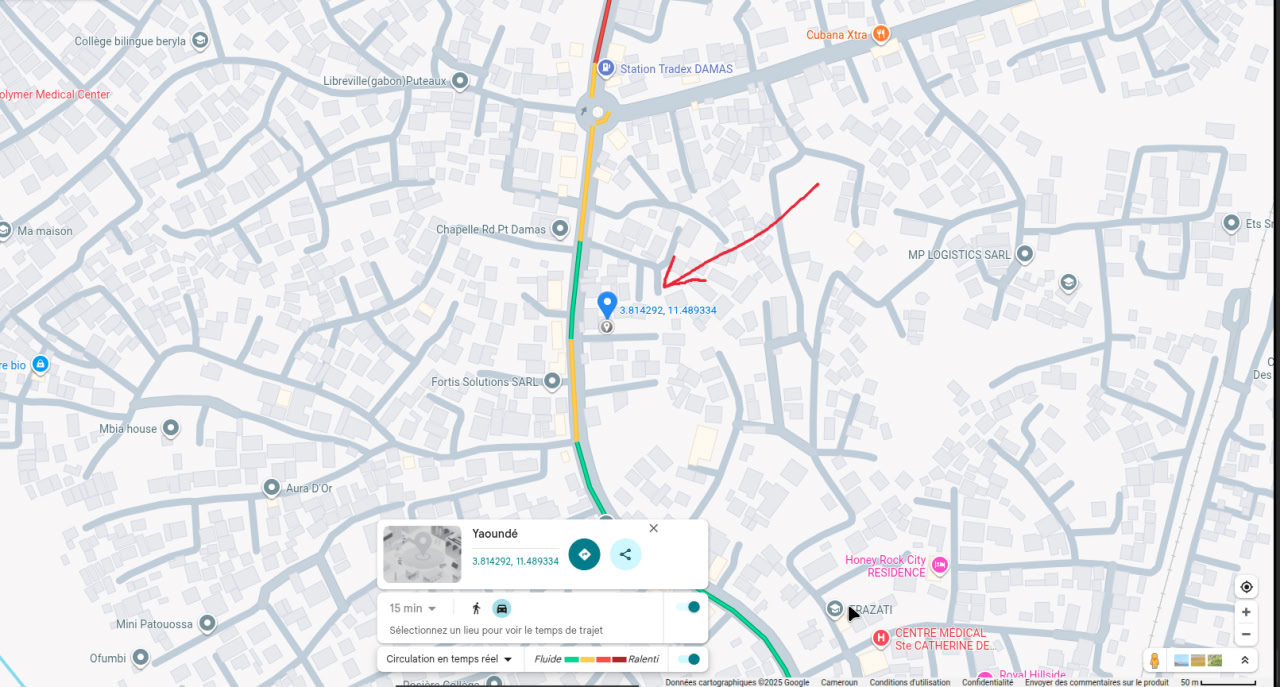
\includegraphics[width=\textwidth, height=12cm]{Images/localisation.jpg}
        \caption{Localisation GPS de KAIROS}
    \end{figure}
    
    \subsection{Mission et vision}
    
    \textbf{Mission :} Kairos analyse les besoins de ses clients, propose des solutions globales adaptées et pilote leur déploiement dans le respect des délais, de la qualité et des coûts.
    
    \textbf{Vision :} Devenir le partenaire de référence des organisations camerounaises et régionales dans leur transformation numérique et l'optimisation de leurs processus documentaires.
    
    \subsection{Domaines d'activité et services}
    
    Kairos propose une gamme complète de services structurés autour de plusieurs axes :
    
    \subsubsection{Audit et conseil}
    L'entreprise offre des prestations d'audit managérial et d'audit documentaire pour aider ses clients à atteindre leurs objectifs. Elle élabore des supports de gouvernance et fournit des conseils pour maintenir la qualité et la sécurité des données et documents.
    
    \subsubsection{Veille stratégique}
    Kairos propose des analyses et des rapports sur les informations et tendances sectorielles, permettant aux clients de prendre des décisions éclairées. L'entreprise met en place des systèmes de veille stratégique performants au sein des organisations.
    
    \subsubsection{Développement numérique}
    L'équipe de développeurs expérimentés accompagne les clients depuis le cahier des charges jusqu'à l'exploitation des solutions. Kairos propose des développements d'applications mobiles sur mesure, la création de sites web d'entreprise ergonomiques et le développement d'applications web innovantes.
    
    \subsubsection{Gestion documentaire et archivage}
    L'entreprise offre des services d'archivage physique et électronique avec des solutions sur mesure pour répondre aux besoins spécifiques de chaque client. Les services incluent également la sauvegarde et la restauration pour garantir la protection des données.
    
    \subsubsection{Formation et accompagnement}
    Kairos propose deux approches : la formation des personnels cibles dans ses métiers et l'accompagnement des équipes pour l'optimisation de leurs pratiques. Les missions incluent le renforcement des parcours professionnels, l'adaptation aux évolutions métier et l'accompagnement des changements organisationnels.
    
    \subsubsection{Gestion de projet}
    L'entreprise accompagne ses clients tout au long du cycle de projet avec une démarche d'accompagnement agile et efficace, gage de réussite pour les projets les plus complexes.
    
    \subsection{Organigramme}
    
    À la tête de l'entreprise Kairos se trouve une Directrice nommée par le conseil d'administration, choisie pour son expertise dans le domaine de la documentation et de l'archivage, sa vision stratégique et sa capacité à diriger une structure spécialisée. Elle est assistée de cinq collaborateurs directs qui pilotent l'ensemble des activités de l'entreprise.
    
    L'organisation s'articule autour d'une équipe de direction composée de :
    \begin{itemize}
        \item \textbf{Directrice} : Direction générale et vision stratégique
        \item \textbf{Attachée de direction} : Support à la direction et coordination
        \item \textbf{Responsable des opérations} : Pilotage des activités opérationnelles
        \item \textbf{Responsable commercial} : Développement commercial et relation client
        \item \textbf{Responsable administratif} : Gestion administrative et financière
        \item \textbf{Coordonnateur des services} : Coordination inter-services
    \end{itemize}
    
    Cette structure permet une organisation efficace autour de trois divisions principales : Kairos Engineering, Kairos Business et Kairos Training Center qui relèvent du Responsable des opérations. Comme le montre l'organigramme ci-dessous, l'entreprise est structurée en trois niveaux hiérarchiques clairs, avec plusieurs services spécialisés sous la supervision de chaque responsable.
    
    \vspace{1cm}
    \begin{figure}[H]
        \centering
        \centerline{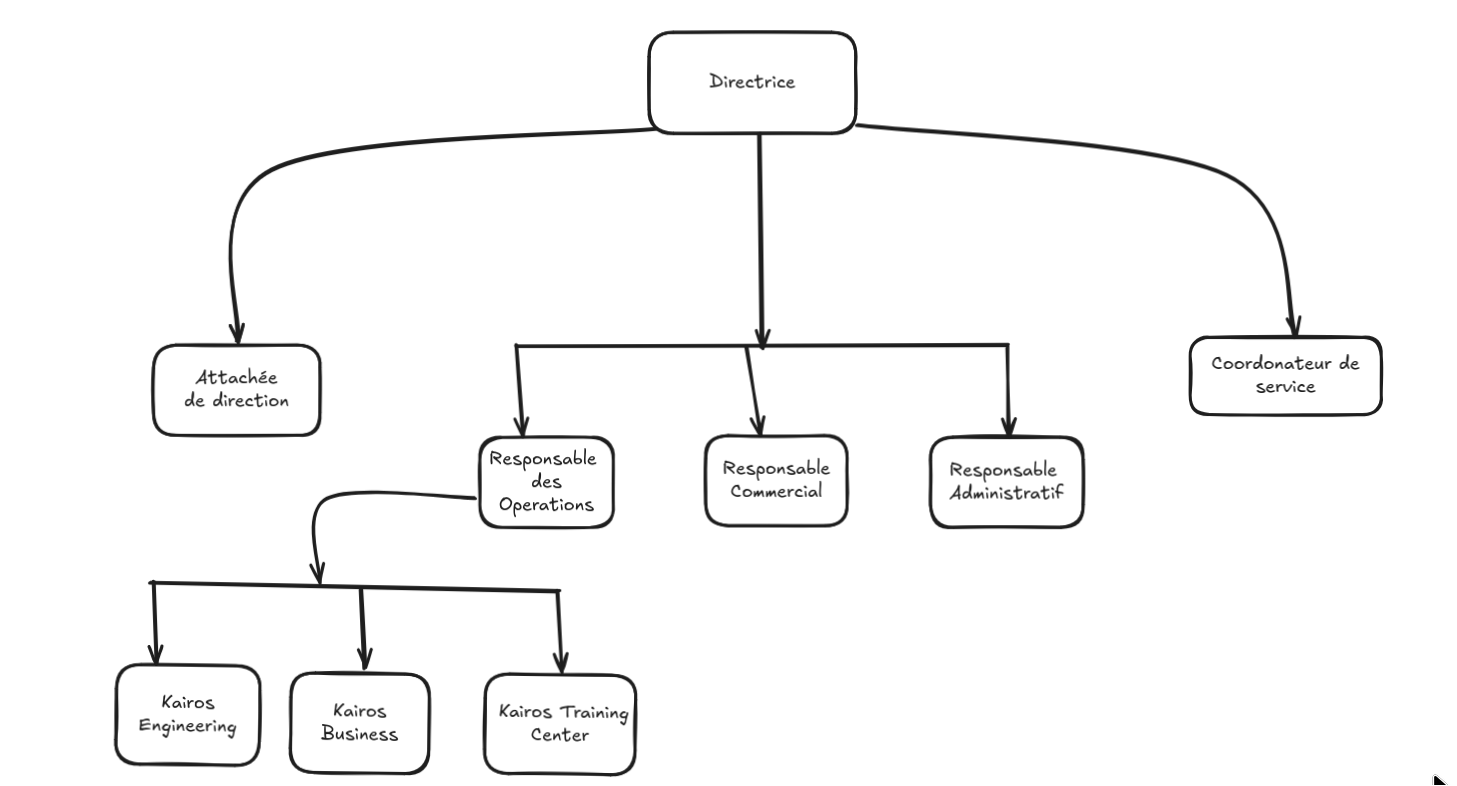
\includegraphics[width=1\linewidth]{Images/org2.png}}
        \caption{Organigramme de l'entreprise KAIROS}
        \label{fig:organigramme_kairos}
    \end{figure}

\section{Déroulement du stage et tâches effectuées}

    \subsection{Accueil et intégration}
    
    Mon intégration au sein de Kairos s'est déroulée de manière progressive et structurée. Dès les premiers jours, j'ai été présenté aux différents services et aux membres de l'équipe, permettant une compréhension globale de l'organisation et des enjeux de l'entreprise.
    
    L'accueil chaleureux et professionnel de l'équipe a facilité mon adaptation à l'environnement de travail. Un plan d'intégration avait été préparé, incluant la présentation des outils, des processus internes et des projets en cours. Cette phase d'accueil m'a également permis de mieux cerner les spécificités du département de documentation et d'archivage, lieu principal de mon stage.
    
    \subsection{Missions et tâches réalisées}
    
    Pendant le déroulement de mon stage, j'ai eu à effectuer plusieurs tâches dans le domaine de la gestion documentaire et du développement d'applications, me permettant de développer mes compétences et de contribuer concrètement aux projets de l'entreprise :
    \begin{table}[H]
        \centering
        \begin{tabularx}{\textwidth}{|l|>{\raggedright\arraybackslash}X|>{\raggedright\arraybackslash}X|}
            \hline
            \textbf{PÉRIODE} & \textbf{TACHES} & \textbf{DESCRIPTION} \\
            \hline
            Première semaine & Observation et analyse des processus & Identification des flux documentaires existants et des points d'amélioration potentiels \\
            \hline
            Deux premières semaines & Configuration de l'environnement de développement & Préparation et installation des outils et technologies nécessaires au projet BPMN \\
            \hline
            Du 15 avril au 30 juin 2024 & Implémentation de la solution BPMN & Développement de l'application \\
            % \hline
            % Tout au long du stage & Tests et validation & Vérification de la conformité de l'application aux besoins fonctionnels du projet \\
            \hline
            Fin de stage & Documentation et transfert & Rédaction de la documentation technique et formation des utilisateurs finaux \\
            \hline
        \end{tabularx}
        \caption{Déroulement détaillé du stage}
        \label{tab:deroulement_stage}
    \end{table}
    
    \subsection{Environnement technologique et apprentissages}
    
    L'environnement technique de Kairos m'a offert l'opportunité de travailler avec des technologies modernes et des outils professionnels. Le département de documentation et d'archivage utilise des solutions variées pour gérer les flux documentaires, ce qui m'a permis de mieux comprendre les enjeux de l'automatisation des processus métier.
    
    Cette expérience m'a également permis d'approfondir mes compétences en analyse de processus, en modélisation BPMN et en développement d'applications métier. La diversité des projets menés par Kairos m'a donné une vision globale des défis liés à la transformation numérique des organisations.

\section{Contexte du projet de fin d'études}

    \subsection{Problématique identifiée}
    
    Au cours de mon stage, j'ai observé que les processus documentaires de Kairos, bien qu'efficaces, présentaient des opportunités d'optimisation significatives. La gestion manuelle de certains flux de travail générait des délais de traitement et des risques d'erreur qui pouvaient être considérablement réduits grâce à une approche d'automatisation.
    
    Les principales difficultés identifiées concernent :
    \begin{itemize}
        \item La traçabilité limitée des documents dans leur cycle de vie
        \item Les redondances dans les processus de validation
        \item Les délais de traitement variables selon la charge de travail
        \item La difficulté de suivi en temps réel de l'avancement des dossiers
    \end{itemize}
    
    \subsection{Opportunité d'amélioration}
    
    L'identification de cette problématique a conduit à la définition de mon projet de fin d'études : développer une application de modélisation et d'automatisation des processus métier utilisant la notation BPMN (Business Process Model and Notation). Cette solution vise à :
    \begin{itemize}
        \item Cartographier les processus documentaires existants
        \item Identifier les goulots d'étranglement et les redondances
        \item Automatiser les tâches répétitives et chronophages
        \item Améliorer la traçabilité des documents et leur suivi
        \item Optimiser les délais de traitement global
        \item Standardiser les procédures documentaires
    \end{itemize}
    
    \subsection{Enjeux stratégiques du projet}
    
    Ce projet répond à plusieurs enjeux stratégiques majeurs pour Kairos :
    
    \textbf{Efficacité opérationnelle :} Réduction significative des temps de traitement des dossiers documentaires et optimisation de l'allocation des ressources humaines.
    
    \textbf{Qualité et fiabilité :} Minimisation des erreurs humaines grâce à l'automatisation des contrôles et des validations.
    
    \textbf{Traçabilité et conformité :} Amélioration du suivi des processus et facilitation des audits de conformité.
    
    \textbf{Évolutivité :} Mise en place d'une architecture flexible capable de s'adapter aux changements organisationnels futurs.
    
    \textbf{Compétitivité :} Positionnement de Kairos comme précurseur dans l'automatisation des processus documentaires au Cameroun.

% \section*{Conclusion}

% L'entreprise Kairos offre un environnement professionnel riche et stimulant, propice au développement de compétences techniques et managériales. La diversité de ses activités et son positionnement stratégique sur le marché de la transformation numérique en font un cadre idéal pour mener un projet d'envergure tel que celui que j'ai entrepris.

% Cette expérience de stage m'a permis de mieux comprendre les enjeux réels des entreprises en matière de gestion documentaire et d'automatisation des processus. Elle constitue le fondement solide de mon projet de fin d'études, dont les chapitres suivants détailleront les aspects techniques, méthodologiques et les résultats obtenus.

% La problématique identifiée chez Kairos illustre parfaitement les défis auxquels font face de nombreuses organisations dans leur quête d'efficacité et de digitalisation. Mon projet s'inscrit donc dans une démarche d'amélioration continue et d'innovation, valeurs chères à l'entreprise d'accueil et essentielles pour son développement futur.
\chapter{État de l'art et analyse des solutions BPMN existantes}
\label{ch:etat_art_bpmn}

Après avoir présenté l'environnement professionnel et le cadre de stage chez Kairos dans le chapitre précédent, ce deuxième chapitre s'attache à explorer l'état de l'art autour de la notation BPMN (Business Process Model and Notation) et des solutions d'automatisation des processus métier. Il vise à analyser les approches existantes, leurs fonctionnalités, ainsi que leurs forces et limites dans le contexte de la modélisation et de l'automatisation des flux documentaires. Pour cela, nous commencerons par définir les concepts fondamentaux liés à BPMN et aux processus métier, puis nous proposerons une analyse comparative des différentes solutions existantes afin de justifier notre approche et les améliorations envisagées.

\section{Concepts fondamentaux et définitions}

\subsection{Évolution de la modélisation des processus métier}

L'histoire de la modélisation des processus métier remonte aux années \textbf{1960} avec l'émergence des premiers diagrammes de flux dans l'industrie manufacturière. Ces outils visaient à documenter et optimiser les chaînes de production en identifiant les étapes, les décisions et les flux de matières.

Dans les années \textbf{1970-1980}, l'informatisation des entreprises a donné naissance aux premières méthodes de modélisation informatique des processus. Les diagrammes de flux de données (DFD) et les modèles entité-relation ont permis de représenter les systèmes d'information de manière structurée.

Les années \textbf{1990} ont marqué l'avènement du \textbf{Business Process Reengineering (BPR)}, une approche révolutionnaire proposée par Michael Hammer et James Champy. Cette méthodologie visait à repenser radicalement les processus d'entreprise pour améliorer la performance, réduire les coûts et accélérer les délais.

Au début des années \textbf{2000}, l'émergence des technologies web et des architectures orientées services (SOA) a favorisé le développement de langages de modélisation standardisés. C'est dans ce contexte qu'est né \textbf{BPMN (Business Process Model and Notation)} en 2004, développé par la Business Process Management Initiative (BPMI).

En \textbf{2005}, BPMN 1.0 est officiellement publié, offrant pour la première fois un standard unifié pour la modélisation des processus métier. Cette notation graphique a révolutionné la communication entre les analystes métier et les développeurs informatiques.

L'évolution s'est poursuivie avec \textbf{BPMN 2.0} en 2011, intégrant des capacités d'exécution et de standardisation XML, permettant ainsi l'automatisation effective des processus modélisés. Cette version a marqué le passage de la simple documentation à l'exécution automatisée des workflows.

\subsection{Présentation de BPMN}

\textbf{BPMN (Business Process Model and Notation)} est un standard de modélisation graphique qui fournit une notation facilement compréhensible par tous les utilisateurs métier, depuis les analystes qui créent les ébauches initiales des processus jusqu'aux développeurs techniques responsables de l'implémentation de ces processus. BPMN crée un pont standardisé pour combler le fossé de communication entre la conception des processus métier et leur implémentation.

La force de BPMN réside dans sa capacité à représenter de manière visuelle et intuitive des processus complexes tout en conservant la rigueur nécessaire à leur automatisation. Contrairement aux méthodes de documentation traditionnelles, BPMN offre une syntaxe précise et exécutable, permettant de passer directement de la modélisation à l'implémentation technique.

BPMN se distingue par quatre catégories principales d'éléments graphiques :

\begin{itemize}
    \item \textbf{Objets de flux} : Événements, activités et passerelles qui définissent le comportement du processus
    \item \textbf{Objets de connexion} : Flux de séquence, flux de messages et associations qui connectent les éléments
    \item \textbf{Couloirs (Swimlanes)} : Pools et lanes qui organisent les activités selon les responsabilités
    \item \textbf{Artefacts} : Objets de données, groupes et annotations qui enrichissent la compréhension
\end{itemize}

\subsection{Principe de l'automatisation des processus dans les systèmes documentaires}

L'\textbf{automatisation des processus métier} consiste à utiliser la technologie pour exécuter automatiquement des tâches récurrentes selon des règles prédéfinies, réduisant ainsi l'intervention humaine et optimisant l'efficacité opérationnelle. Dans le contexte des systèmes documentaires, cette automatisation présente des enjeux particuliers liés à la gestion, au traitement et au suivi des flux documentaires.

L'automatisation offre de nombreux avantages tant pour les organisations (réduction des délais de traitement, minimisation des erreurs humaines, amélioration de la traçabilité et standardisation des procédures) que pour les utilisateurs (interface simplifiée, notifications automatiques, accès facilité aux informations et suivi en temps réel des dossiers).

Les possibilités offertes par l'automatisation dans le domaine documentaire sont multiples. On peut noter le \textbf{routage intelligent} (permettant l'acheminement automatique des documents selon leur type, leur contenu ou leur priorité), la \textbf{validation automatisée} (contrôles de conformité, vérifications de complétude et application de règles métier), les \textbf{notifications contextuelles} (alertes sur les échéances, notifications de validation et rapports d'avancement), et l'\textbf{archivage programmé} (classement automatique selon des règles prédéfinies et gestion des cycles de vie documentaires).

\section{Classification des solutions BPMN par approche technique}

\subsection{Solutions de modélisation pure (Design-only)}

Les solutions de modélisation pure se concentrent exclusivement sur la création et la documentation de processus métier sans capacité d'exécution. Elles sont principalement destinées aux analystes métier et aux architectes de processus qui souhaitent cartographier, analyser et communiquer autour des workflows organisationnels.

\subsubsection{Lucidchart : la simplicité collaborative}
Lancé en 2008, Lucidchart s'est imposé comme une solution de diagramming en ligne particulièrement appréciée pour sa simplicité d'usage et ses fonctionnalités collaboratives. La plateforme propose des templates BPMN prêts à l'emploi et permet la co-édition en temps réel. Avec plus de 25 millions d'utilisateurs en 2024, Lucidchart séduit par son interface intuitive et ses intégrations avec les outils bureautiques (Google Workspace, Microsoft 365). Cependant, la plateforme présente certaines limitations : absence de validation syntaxique BPMN rigoureuse, fonctionnalités avancées limitées pour la modélisation complexe, et impossibilité d'exporter vers des moteurs d'exécution.

\subsubsection{Draw.io (diagrams.net) : l'alternative open source}
Draw.io, rebaptisé diagrams.net, est une solution de diagramming gratuite et open source développée par JGraph. Elle propose un support BPMN complet avec une bibliothèque d'éléments conforme aux standards. Sa force réside dans sa gratuité totale, son fonctionnement hors ligne possible, et ses multiples options d'intégration (Confluence, GitHub, etc.). Toutefois, l'absence de fonctionnalités collaboratives avancées et de validation BPMN automatisée limite son usage dans des contextes professionnels exigeants.

\subsubsection{Microsoft Visio : la référence professionnelle}
Microsoft Visio demeure une référence dans le domaine de la modélisation de processus, avec un support BPMN robuste et des fonctionnalités avancées de validation. Son intégration native avec l'écosystème Microsoft Office et ses capacités de personnalisation en font un choix privilégié dans les environnements d'entreprise. Néanmoins, son coût élevé, sa courbe d'apprentissage importante et l'absence de capacités d'exécution constituent des freins à son adoption généralisée.

\subsection{Solutions d'exécution de processus (Execution Engines)}

Les moteurs d'exécution BPMN transforment les modèles graphiques en workflows exécutables, permettant l'automatisation effective des processus métier. Ces solutions offrent des environnements runtime capables d'interpréter et d'exécuter les diagrammes BPMN.

\subsubsection{Camunda Platform : l'écosystème complet}
Camunda Platform, créée en 2008 en Allemagne, s'est imposée comme l'une des solutions d'automatisation de processus les plus complètes du marché. La plateforme combine un moteur d'exécution BPMN haute performance, des outils de modélisation intégrés, et un environnement de monitoring avancé. Avec plus de 4 millions de téléchargements de son moteur open source, Camunda séduit par sa robustesse technique, sa conformité stricte aux standards BPMN 2.0, et son écosystème d'extensions. Sa version Community Edition gratuite permet aux organisations de démarrer sans investissement initial. Cependant, la complexité de mise en œuvre, les coûts de licence pour les fonctionnalités avancées, et la nécessité de compétences techniques spécialisées peuvent constituer des obstacles pour certaines organisations.

\subsubsection{Activiti : la flexibilité open source}
Activiti, développé initialement par Alfresco et aujourd'hui maintenu par une communauté active, se positionne comme une alternative open source légère et flexible. Le moteur d'exécution Java offre une API riche et des possibilités d'intégration étendues. Sa force réside dans sa simplicité de déploiement, sa documentation complète, et sa communauté active. Toutefois, Activiti présente des limitations en termes d'outils de monitoring, d'interface utilisateur intégrée, et de support commercial par rapport aux solutions commerciales.

\subsubsection{jBPM : l'intégration Red Hat}
jBPM, développé par Red Hat, propose un framework complet de gestion de processus métier intégré à l'écosystème JBoss. La solution se distingue par ses capacités de règles métier avancées, son intégration avec les technologies Red Hat, et ses fonctionnalités de gestion de cas (Case Management). Néanmoins, sa dépendance à l'écosystème Red Hat, sa courbe d'apprentissage prononcée, et ses performances parfois moindres sur de gros volumes constituent des points de vigilance.

\subsection{Solutions intégrées (All-in-One)}

Les plateformes intégrées combinent modélisation, exécution, monitoring et optimisation des processus dans un environnement unifié. Elles visent à offrir une expérience utilisateur complète pour la gestion du cycle de vie des processus.

\subsubsection{Signavio : la plateforme d'entreprise}
Signavio, acquis par SAP en 2021, propose une suite complète de gestion des processus métier dans le cloud. La plateforme intègre des outils de modélisation collaboratifs, d'analyse de conformité, et d'optimisation des processus. Avec plus de 1 million d'utilisateurs dans le monde, Signavio se distingue par ses capacités d'analyse avancées, ses fonctionnalités de gouvernance des processus, et son intégration avec SAP. Cependant, les coûts de licence élevés, la dépendance au cloud, et la complexité de paramétrage limitent son accessibilité aux grandes organisations.

\subsubsection{Bizagi : l'accessibilité métier}
Bizagi se positionne comme une plateforme accessible aux utilisateurs métier, avec des interfaces low-code et des assistants de création simplifiés. La solution propose un environnement complet de modélisation, exécution et analyse des processus. Sa force réside dans sa facilité d'utilisation, ses templates sectoriels, et ses capacités d'intégration mobile. Toutefois, les limitations en termes de personnalisation avancée, de performance sur de gros volumes, et de flexibilité technique peuvent constituer des freins pour des besoins complexes.

\subsubsection{Nintex : l'intégration SharePoint}
Nintex s'est spécialisé dans l'automatisation de processus pour l'écosystème Microsoft, avec une intégration native à SharePoint et Office 365. La plateforme propose des outils de création de workflows visuels et des fonctionnalités de gestion documentaire intégrées. Son principal atout réside dans son intégration transparente avec les outils Microsoft utilisés en entreprise. Cependant, sa dépendance à l'écosystème Microsoft, ses coûts de licence croissants, et ses limitations en termes de standards BPMN stricts constituent des points de vigilance.

\section{Classification par domaine d'application}

\subsection{Solutions orientées gestion documentaire}

Les solutions spécialisées dans la gestion documentaire intègrent des fonctionnalités BPMN pour automatiser les workflows liés aux documents, leur validation, leur routage et leur archivage.

\subsubsection{Alfresco Process Services : la gestion de contenu processuelle}
Alfresco Process Services combine gestion de contenu d'entreprise (ECM) et automatisation de processus BPMN. La solution permet de créer des workflows documentaires sophistiqués avec gestion des versions, contrôle d'accès, et traçabilité complète. Son intégration native avec Alfresco Content Services offre un environnement unifié pour la gestion du cycle de vie documentaire. Cependant, la complexité de déploiement, les coûts de licence, et la nécessité de compétences spécialisées peuvent constituer des obstacles pour les organisations de taille moyenne.

\subsubsection{OnBase by Hyland : l'automatisation de processus documentaires}
OnBase propose une plateforme complète de gestion de l'information d'entreprise avec des capacités d'automatisation de processus avancées. La solution excelle dans la capture automatique de documents, le routage intelligent basé sur le contenu, et l'intégration avec les systèmes existants. Sa force réside dans ses capacités de reconnaissance optique de caractères (OCR), ses fonctionnalités de signature électronique, et ses outils d'audit complets. Néanmoins, les investissements importants requis et la complexité de paramétrage limitent son adoption aux grandes organisations.

\subsubsection{SharePoint Workflows : l'intégration Microsoft}
Les workflows SharePoint permettent d'automatiser les processus documentaires au sein de l'écosystème Microsoft. La solution propose des outils de création visuelle de workflows et s'intègre naturellement avec Office 365. Bien que moins sophistiquée que les solutions spécialisées, elle offre une approche pragmatique pour les organisations déjà équipées de technologies Microsoft. Toutefois, les limitations en termes de complexité des processus, de monitoring avancé, et de conformité BPMN stricte peuvent nécessiter des solutions complémentaires.

\subsection{Solutions orientées RH et approbations}

Ces solutions se spécialisent dans l'automatisation des processus de ressources humaines, de validation hiérarchique et de gestion des demandes internes.

\subsubsection{BambooHR Workflows : l'automatisation RH simplifiée}
BambooHR intègre des fonctionnalités de workflow pour automatiser les processus RH courants : demandes de congés, évaluations de performance, intégration de nouveaux employés. La solution se distingue par sa simplicité d'usage et son intégration complète avec le SIRH. Cependant, les possibilités de personnalisation limitées et l'absence de support BPMN standard peuvent constituer des freins pour des processus complexes.

\subsubsection{ServiceNow HR Service Delivery : la plateforme d'entreprise}
ServiceNow propose une plateforme complète d'automatisation des services RH avec des capacités de workflow avancées. La solution offre des outils de création de processus sophistiqués, des intégrations étendues, et des fonctionnalités d'analyse de performance. Son écosystème riche et ses capacités d'extension en font une solution de choix pour les grandes organisations. Toutefois, la complexité de mise en œuvre et les coûts élevés limitent son accessibilité.

\subsubsection{Zapier : l'automatisation accessible}
Zapier démocratise l'automatisation en proposant une approche no-code pour connecter différentes applications et automatiser des tâches simples. Bien que ne supportant pas nativement BPMN, la solution permet de créer des workflows basiques d'approbation et de notification. Sa force réside dans ses milliers d'intégrations prêtes à l'emploi et sa simplicité d'usage. Cependant, les limitations en termes de logique complexe, de gestion d'erreurs, et de monitoring professionnel la cantonnent aux besoins simples.

\subsection{Solutions sectorielles spécialisées}

Certaines solutions BPMN se spécialisent dans des secteurs d'activité spécifiques, offrant des fonctionnalités et des templates adaptés aux métiers.

\subsubsection{ARIS : la modélisation d'entreprise}
ARIS de Software AG propose une approche globale de la modélisation et de l'optimisation des processus d'entreprise. La solution excelle dans la cartographie des processus complexes, l'analyse de conformité, et la simulation de scénarios. Son approche méthodologique rigoureuse et ses capacités d'analyse avancées en font un choix privilégié pour les grandes organisations industrielles. Néanmoins, la complexité de la solution, les coûts importants, et la nécessité de formation spécialisée limitent son adoption.

\subsubsection{Pega Platform : l'automatisation intelligente}
Pega Platform combine BPM, gestion de cas, et intelligence artificielle pour offrir une automatisation intelligente des processus. La solution se distingue par ses capacités de prise de décision automatisée, ses fonctionnalités de machine learning intégrées, et son approche centrée sur l'expérience client. Particulièrement prisée dans les secteurs bancaire et assurantiel, elle offre des accélérateurs sectoriels et des frameworks prêts à l'emploi. Cependant, la complexité technique, les coûts de licence élevés, et la courbe d'apprentissage importante constituent des obstacles significatifs.

\section{Analyse comparative et synthèse}

\subsection{Critères d'évaluation des solutions}

Pour évaluer objectivement les différentes solutions BPMN, nous avons défini plusieurs critères clés :

\textbf{Conformité aux standards :} Respect des spécifications BPMN 2.0, capacité d'import/export, validation syntaxique.

\textbf{Facilité d'utilisation :} Interface intuitive, courbe d'apprentissage, documentation, support.

\textbf{Capacités d'exécution :} Moteur de workflow, gestion des données, intégrations, performance.

\textbf{Fonctionnalités avancées :} Monitoring, analytics, optimisation, gouvernance.

\textbf{Coût total de possession :} Licences, déploiement, maintenance, formation.

\textbf{Évolutivité :} Capacité de montée en charge, extensibilité, pérennité.

\subsection{Forces et limites des approches existantes}

L'analyse des solutions existantes révèle plusieurs tendances marquantes :

\textbf{Polarisation des offres :} Le marché se divise entre solutions simples mais limitées et plateformes complètes mais complexes, laissant peu d'options intermédiaires.

\textbf{Coûts prohibitifs :} Les solutions professionnelles présentent souvent des coûts de licence et de déploiement importants, limitant leur accessibilité aux grandes organisations.

\textbf{Complexité technique :} La plupart des solutions d'exécution requièrent des compétences techniques spécialisées, créant une barrière à l'adoption.

\textbf{Manque d'adaptabilité locale :} Peu de solutions proposent des fonctionnalités spécifiquement adaptées aux contextes locaux ou aux petites structures.

\textbf{Intégration limitée :} Les capacités d'intégration avec les systèmes existants restent souvent complexes et coûteuses.

\subsection{Opportunités d'innovation identifiées}

Cette analyse révèle plusieurs opportunités d'innovation non pleinement exploitées :

\textbf{Simplification de l'usage :} Développer des interfaces plus intuitives permettant aux utilisateurs métier de créer et modifier des processus sans formation technique approfondie.

\textbf{Coût d'entrée réduit :} Proposer des solutions accessibles aux PME et structures de taille intermédiaire, avec des modèles de tarification adaptés.

\textbf{Adaptabilité contextuelle :} Intégrer des fonctionnalités d'adaptation aux spécificités locales, réglementaires et organisationnelles.

\textbf{Approche progressive :} Permettre une adoption graduelle avec des fonctionnalités de base extensibles selon les besoins.

\textbf{Intégration facilitée :} Simplifier les processus d'intégration avec les systèmes existants grâce à des connecteurs prêts à l'emploi.

\subsection{Synthèse critique}

L’analyse fait ressortir plusieurs constats :

\begin{itemize}
    \item \textbf{Polarisation du marché} : solutions très simples mais limitées (Lucidchart, Draw.io) ou très puissantes mais complexes (Camunda, Signavio).
    \item \textbf{Barrière économique} : les coûts de licence sont souvent prohibitifs pour les PME.
    \item \textbf{Barrière technique} : la mise en œuvre de moteurs BPMN exige des compétences spécialisées.
    \item \textbf{Manque d’adaptabilité} : peu de solutions sont pensées pour des contextes locaux ou des projets de taille intermédiaire.
\end{itemize}

L’état de l’art met en évidence une lacune entre les solutions \textit{trop simples pour être exécutables} et celles \textit{trop complexes et coûteuses pour être accessibles}. Peu d’outils permettent de concilier simplicité d’utilisation, conformité BPMN 2.0, intégration facile et coûts maîtrisés.

C’est dans cette perspective que nous proposons une solution innovante basée sur une architecture légère intégrant \textbf{Spring Boot} (moteur et backend) et \textbf{React} (interface utilisateur). Notre approche vise à offrir un outil adaptable, extensible et accessible, capable de répondre aux besoins de modélisation et d’automatisation dans un contexte organisationnel local. Cette proposition sera détaillée dans le chapitre suivant.


\chapter{Architecture et conception technique de Harmoni}
\label{ch:conception_harmoni}

Après avoir exploré l'état de l'art des solutions BPMN existantes, ce chapitre présente la conception de \textbf{Harmoni}, l'application de modélisation et d'automatisation des processus métier BPMN développée dans le cadre de ce projet. 
L'objectif est de détailler :
\begin{itemize}
    \item l'analyse des besoins (fonctionnels et non fonctionnels),
    \item la conception fonctionnelle avec diagrammes UML,
    \item l'architecture technique et la structure des composants.
\end{itemize}

\section{Analyse des besoins}

\subsection{Besoins fonctionnels}
Les besoins fonctionnels définissent les services que doit rendre l'application Harmoni :
\begin{itemize}
    \item Permettre la modélisation graphique de processus métier en notation BPMN 2.0.
    \item Assurer la validation syntaxique et la sauvegarde des modèles.
    \item Exécuter automatiquement des workflows via un moteur BPMN.
    \item Intégrer les processus automatisés aux systèmes documentaires existants de Kairos.
    \item Fournir un tableau de bord de monitoring en temps réel des processus exécutés.
    \item Gérer les utilisateurs, rôles et droits d’accès (gestionnaires de processus, utilisateurs finaux).
\end{itemize}

\subsection{Besoins non fonctionnels}
Les besoins non fonctionnels fixent les contraintes de performance, de sécurité et de maintenabilité :
\begin{itemize}
    \item \textbf{Performance} : temps de réponse inférieur à 2 secondes pour les opérations critiques.
    \item \textbf{Scalabilité} : support de plusieurs centaines d’instances de processus simultanées.
    \item \textbf{Sécurité} : authentification par JWT, communications chiffrées en HTTPS.
    \item \textbf{Interopérabilité} : respect du standard BPMN 2.0 et API REST pour intégration.
    \item \textbf{Fiabilité} : gestion robuste des erreurs et reprise après panne.
    \item \textbf{Ergonomie} : interface intuitive adaptée aux utilisateurs métier non techniques.
\end{itemize}

\section{Conception fonctionnelle}

\subsection{Diagramme de cas d’utilisation}
La figure~\ref{fig:uc_bpmn_app} présente les principaux acteurs et cas d'utilisation de la plateforme.  
\begin{figure}[h]
    \centering
    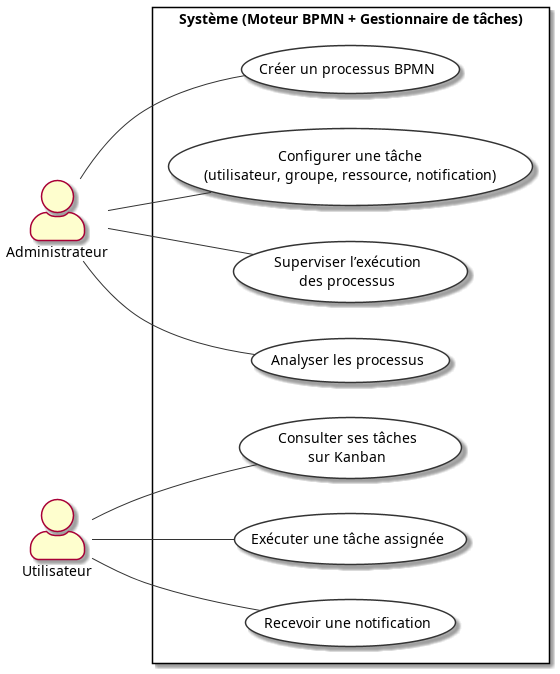
\includegraphics[width=0.9\textwidth]{Images/usecase.png}
    \caption{Diagramme de cas d'utilisation — Application BPMN}
    \label{fig:uc_bpmn_app}
\end{figure}

\subsection{Diagramme de classes}
Le diagramme de classes met en évidence les entités principales (Processus, Tâche, Utilisateur, Document, Notification, etc.) et leurs relations (voir Figure~\ref{fig:class_bpmn_app}).  
% \begin{figure}[h]
%     \centering
%     \includegraphics[width=0.9\textwidth]{Images/class.png}
%     \caption{Diagramme de classes — Modèle conceptuel de Harmoni}
%     \label{fig:class_bpmn_app}
% \end{figure}

\subsection{Diagramme de séquence}
La figure~\ref{fig:seq_exec_bpmn} illustre une séquence représentative d'exécution d'un processus BPMN par un utilisateur, depuis la modélisation jusqu’au monitoring.
\begin{figure}[h]
    \centering
    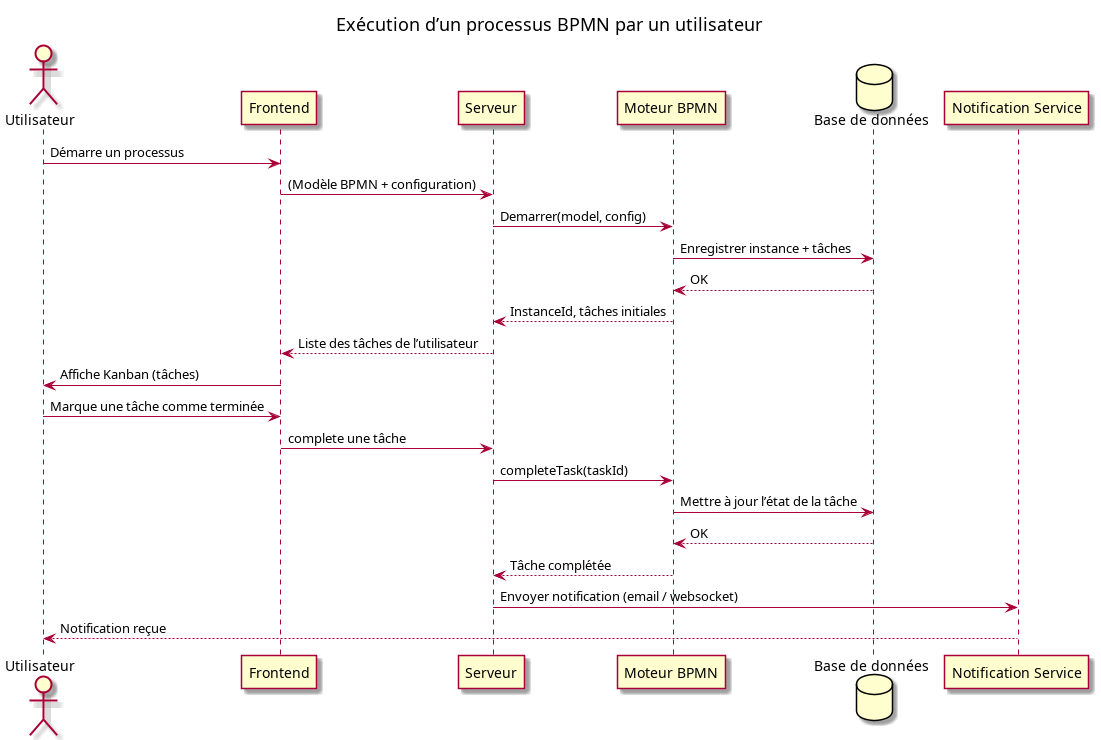
\includegraphics[width=0.95\textwidth]{Images/sequence.png}
    \caption{Diagramme de séquence — Exécution d’un processus BPMN par un utilisateur}
    \label{fig:seq_exec_bpmn}
\end{figure}

\section{Structure des composants et dépendances}

\subsection{Schéma directeur de Harmoni}
Cette section présente l'architecture globale de Harmoni et les flux principaux entre les composants.
\begin{figure}[h]
    \centering
    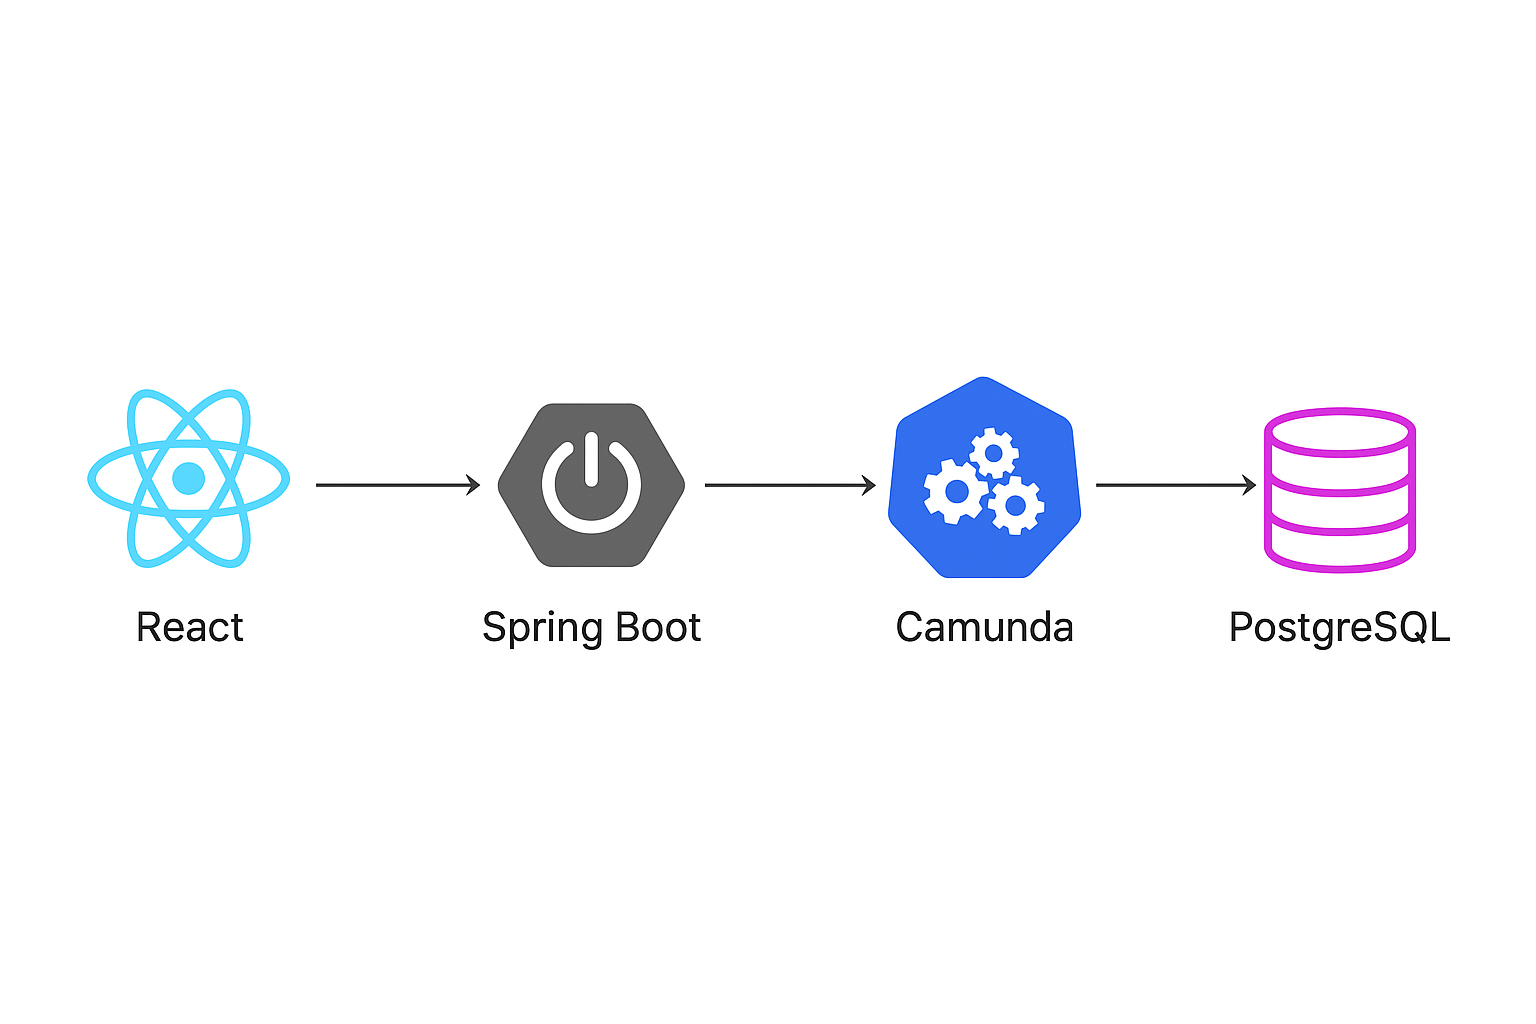
\includegraphics[width=0.8\textwidth]{Images/Architecture.png}
    \caption{Architecture globale de Harmoni}
    \label{fig:harmoni_global_architecture}
\end{figure}

\subsection{Choix de l’architecture}
Cette sous-section détaille les couches (React, API Spring Boot, Moteur BPMN, Intégrations) et leurs responsabilités.

\subsection{Flux de données et interactions}
Synthèse des échanges entre frontend, API, moteur BPMN et systèmes documentaires.

\section{Implémentation technique}

\subsection{Le cœur logique de Harmoni}
(== ton texte existant sur l’architecture Spring Boot, API REST, sécurité, moteur BPMN ==)

\subsection{L’interface utilisateur React}
(== ton texte existant sur l’éditeur BPMN, React, monitoring, etc. ==)

---

\chapter{Mise en œuvre et déploiement de Harmoni}
\label{ch:mise_oeuvre_harmoni}

Cette phase décrit la mise en œuvre pratique de la solution Harmoni développée. Elle présente la liste du matériel et des logiciels nécessaires, les étapes de déploiement de l'application d'automatisation BPMN, ainsi qu'une analyse du coût de réalisation du projet dans le contexte de l'optimisation des processus documentaires chez Kairos.

\section{Choix des outils et technologies}

\subsection{Frontend : React}

Pour le frontend, React a été choisi pour les raisons décrites ci-dessous après une évaluation des technologies les plus utilisées côté interface utilisateur web.

\begin{table}[H]
    \centering
    \resizebox{\textwidth}{!}{
        \begin{tabular}{|p{3cm}|p{5cm}|p{5cm}|p{5cm}|}
            \hline
            \textbf{Nom} & \textbf{React} & \textbf{Vue.js} & \textbf{Angular} \\
            \hline
            % Description & Bibliothèque JavaScript pour interfaces utilisateur avec composants réutilisables & Framework progressif JavaScript, simple et flexible & Framework complet TypeScript avec architecture MVC \\
            % \hline
            Langage & JavaScript/TypeScript & JavaScript/TypeScript & TypeScript \\
            \hline
            Performances & Excellentes grâce au Virtual DOM et à l'optimisation des re-rendus & Très bonnes, légère et rapide & Bonnes, mais plus lourd pour les petites applications \\
            \hline
            Écosystème & Énorme écosystème, nombreuses bibliothèques pour BPMN (bpmn-js) & Écosystème solide mais plus restreint & Écosystème complet intégré \\
            \hline
            Courbe d'apprentissage & Modérée, concepts JSX et hooks à maîtriser & Douce, syntaxe proche du HTML classique & Abrupte, architecture complexe et TypeScript obligatoire \\
            \hline
        \end{tabular}
    }
    \caption{Comparaison des technologies frontend}
    \label{tab:comparatif-frontend}
\end{table}

\subsubsection{Pourquoi utiliser React ?}
\begin{dinglist}{80}
    \item Excellente intégration avec les bibliothèques BPMN comme bpmn-js pour l'édition graphique de processus.
    \item Architecture composant facilitant la création d'interfaces complexes pour la modélisation BPMN.
    \item Large communauté et écosystème riche permettant de trouver rapidement des solutions aux problèmes spécifiques.
    \item Performance optimale pour les applications interactives avec mise à jour en temps réel des processus.
    \item Support TypeScript natif pour un développement plus robuste et maintenable.
\end{dinglist}

\begin{figure}[H]
    \centering
    
\includegraphics[width=0.3\textwidth]{Images/react.png}
    \caption{React}
    \label{fig:react}
\end{figure}

\subsection{Backend : Spring Boot}

Pour le développement du backend de l'application, Spring Boot a été utilisé pour la conception des API REST et l'intégration du moteur BPMN. Le tableau ci-dessous justifie notre choix.

\begin{table}[H]
    \centering
    \resizebox{\textwidth}{!}{
        \begin{tabular}{|p{3cm}|p{5cm}|p{5cm}|p{5cm}|}
            \hline
            \textbf{Nom} & \textbf{Spring Boot} & \textbf{Node.js Express} & \textbf{Laravel} \\
            \hline
            Description & Framework Java robuste avec écosystème complet, excellent pour applications d'entreprise & Framework JavaScript minimaliste et rapide pour API REST & Framework PHP moderne avec fonctionnalités intégrées \\
            \hline
            Langage & Java & JavaScript & PHP \\
            \hline
            Intégration BPMN & Excellente avec Camunda, Flowable, Activiti natifs & Possible mais nécessite des adaptateurs & Support limité, intégrations tierces \\
            \hline
            Performance & Très haute performance, compilation optimisée & Excellente pour I/O intensif & Bonne performance pour applications web \\
            \hline
            % Écosystème & Écosystème mature spécialisé BPM, Spring Security, Spring Data & Large écosystème JavaScript mais fragmenté & Écosystème PHP riche mais moins orienté BPM \\
            % \hline
            Scalabilité & Excellente scalabilité horizontale et verticale & Bonne scalabilité avec clustering & Scalabilité correcte avec optimisations \\
            \hline
        \end{tabular}
    }
    \caption{Comparaison des technologies backend}
    \label{tab:comparatif-backend}
\end{table}

\subsubsection{Pourquoi utiliser Spring Boot ?}
\begin{dinglist}{80}
    \item Intégration native parfaite avec les moteurs BPMN (Camunda, Flowable) pour l'automatisation des processus.
    \item Architecture robuste et sécurisée adaptée aux environnements d'entreprise comme Kairos.
    \item Spring Security pour une gestion avancée de l'authentification et des autorisations.
    \item Écosystème Spring complet (Data, Cloud, Batch) facilitant l'intégration avec les systèmes existants.
    \item Performance élevée et gestion optimisée des ressources pour les applications BPMN intensives.
\end{dinglist}

\begin{figure}[H]
    \centering
    
\includegraphics[width=0.5\textwidth]{Images/spring_boot.png}
    \caption{Spring Boot}
    \label{fig:spring_boot}
\end{figure}

\subsection{Base de données : PostgreSQL}

PostgreSQL a été choisi pour les raisons décrites ci-dessous après une évaluation des technologies de base de données pertinentes pour les applications BPMN.

\begin{table}[H]
    \centering
    \resizebox{\textwidth}{!}{
        \begin{tabular}{|p{4cm}|p{5cm}|p{5cm}|p{5cm}|}
            \hline
            \textbf{Nom} & \textbf{PostgreSQL} & \textbf{MySQL} & \textbf{MongoDB} \\
            \hline
            Description & SGBD relationnel avancé, open source, support JSON natif & SGBD relationnel populaire, rapide et fiable & Base NoSQL orientée documents \\
            \hline
            % Support BPMN & Excellent pour métadonnées processus, historique, JSON pour configuration & Bon support relationnel classique & Pas adapté aux structures BPMN relationnelles \\
            % \hline
            Performances & Excellentes pour requêtes complexes et analytiques & Très bonnes pour requêtes simples & Excellentes pour données non-structurées \\
            \hline
            Transactions & Support ACID complet, transactions complexes & Support ACID, transactions standards & Pas de transactions multi-documents (versions récentes seulement) \\
            \hline
            % Extensibilité & Très extensible, types personnalisés, fonctions & Extensibilité limitée & Très flexible pour schémas évolutifs \\
            % \hline
            Intégration Spring & Support natif JPA/Hibernate excellent & Support natif standard & Support Spring Data MongoDB \\
            \hline
        \end{tabular}
    }
    \caption{Tableau comparatif des bases de données}
    \label{tab:comparatif-bd}
\end{table}

\subsubsection{Pourquoi utiliser PostgreSQL ?}
\begin{dinglist}{80}
    \item Support natif JSON pour stocker les configurations BPMN complexes et les données de processus.
    \item Excellente performance pour les requêtes analytiques sur l'historique des processus et le monitoring.
    \item Support ACID complet essentiel pour l'intégrité des données dans les workflows critiques.
    \item Extensibilité avancée permettant des types de données personnalisés pour les métadonnées BPMN.
    \item Intégration parfaite avec Spring Boot et les moteurs BPMN pour la persistance des processus.
\end{dinglist}

\begin{figure}[H]
    \centering
    
\includegraphics[width=0.3\textwidth]{Images/postgresql.png}
    \caption{PostgreSQL}
    \label{fig:postgresql}
\end{figure}

\subsection{Moteur BPMN : Camunda}

Pour l'exécution des processus BPMN, Camunda a été intégré comme moteur d'automatisation des workflows documentaires.

\begin{table}[H]
    \centering
    \resizebox{\textwidth}{!}{
        \begin{tabular}{|p{3cm}|p{5cm}|p{5cm}|p{5cm}|}
            \hline
            \textbf{Nom} & \textbf{Camunda} & \textbf{Flowable} & \textbf{Activiti} \\
            \hline
            Description & Plateforme BPM complète avec moteur robuste et outils intégrés & Moteur BPMN léger, fork d'Activiti avec améliorations & Moteur historique, plus simple mais fonctionnalités limitées \\
            \hline
            Intégration Spring & Starter Spring Boot natif, configuration automatique & Bonne intégration Spring Boot & Intégration Spring standard \\
            \hline
            Monitoring & Interface web complète, métriques avancées & Interface basique, métriques standards & Interface simple, monitoring limité \\
            \hline
            Performance & Très haute performance, optimisé pour la production & Bonne performance, plus léger & Performance correcte pour charges modérées \\
            \hline
            Documentation & Documentation exhaustive, communauté active & Documentation correcte & Documentation basique \\
            \hline
        \end{tabular}
    }
    \caption{Comparaison des moteurs BPMN}
    \label{tab:comparatif-bpmn-engines}
\end{table}

\subsubsection{Pourquoi utiliser Camunda ?}
\begin{dinglist}{80}
    \item Moteur BPMN 2.0 le plus mature et robuste du marché, adapté aux environnements de production.
    \item Intégration Spring Boot native avec configuration automatique et starter dédié.
    \item Extensibilité excellente pour les connecteurs personnalisés vers les systèmes documentaires existants.
    \item Communauté active et documentation complète facilitant le développement et la maintenance.
\end{dinglist}

\begin{figure}[H]
    \centering
    
\includegraphics[width=0.2\textwidth]{Images/camunda.jpeg}
    \caption{Camunda}
    \label{fig:camunda}
\end{figure}

\section{Présentation de l'environnement de travail}

\subsection{Environnement logiciel}

Cette section décrit les outils et les équipements utilisés pour le développement et le déploiement de l'application Harmoni d'automatisation des processus BPMN.

\subsubsection{Système d'exploitation}
\begin{dinglist}{80}
    \item \textbf{Ubuntu 22.04.3 LTS} : Distribution Linux stable et professionnelle, largement utilisée en environnement de développement et de production. Ubuntu LTS offre une stabilité éprouvée, un support à long terme, une sécurité renforcée, et une compatibilité excellente avec les outils de développement Java et les environnements Docker. Il est particulièrement adapté au développement d'applications Spring Boot et à l'intégration avec les systèmes d'entreprise comme ceux de Kairos.\footnote{Ubuntu, \url{https://ubuntu.com/}}
\end{dinglist}

\begin{figure}[H]
    \centering
    
\includegraphics[width=0.3\textwidth]{Images/ubuntu.png}
    \caption{Ubuntu 22.04.3 LTS}
    \label{fig:ubuntu}
\end{figure}

\subsubsection{Environnement de développement (IDE)}

\paragraph{}{
\begin{dinglist}{80}
    
    \item \textbf{IntelliJ IDEA Ultimate} : IntelliJ IDEA est l'IDE de référence pour le développement Java et Spring Boot. Il offre un support natif excellent pour Spring Framework, une intégration parfaite avec Maven/Gradle, des outils de debugging avancés, et des plugins spécialisés pour le développement BPMN et l'intégration Camunda.
    
    \begin{figure}[H]
        \centering
        
\includegraphics[width=0.2\textwidth]{Images/intelliJ.png}
        \caption{IntelliJ IDEA Ultimate}
        \label{fig:intellij}
    \end{figure}
\end{dinglist}}

\paragraph{}{
\begin{dinglist}{80}
    
    \item \textbf{Visual Studio Code} : Visual Studio Code est utilisé pour le développement React avec d'excellentes extensions pour JavaScript/TypeScript, React, et les outils de développement frontend. Il offre une intégration Git native, un terminal intégré, et des extensions spécialisées pour le développement d'interfaces BPMN.
    
    % Figure for VS Code temporarily disabled: image not found (Images/vs_code.png)
    % \begin{figure}[H]
    %     \centering
    %     \includegraphics[width=0.6\textwidth]{Images/vs_code.png}
    %     \caption{Visual Studio Code}
    %     \label{fig:vscode}
    % \end{figure}
\end{dinglist}}


\subsubsection{Gestionnaire de version et outils de collaboration}

\paragraph{}{
\begin{dinglist}{80}
    
    \item \textbf{Git} : Git est le système de contrôle de version décentralisé utilisé pour le suivi des modifications du code source de Harmoni, permettant la collaboration et la gestion des versions des processus BPMN.
    
    \begin{figure}[H]
        \centering
        
\includegraphics[width=0.2\textwidth]{Images/git.png}
        \caption{Git}
        \label{fig:git}
    \end{figure}
\end{dinglist}}

\subsubsection{Outils de conteneurisation et déploiement}

\paragraph{}{
\begin{dinglist}{80}
    
    \item \textbf{Docker} : Docker est utilisé pour la conteneurisation de l'application Harmoni, permettant un déploiement cohérent et portable sur différents environnements (développement, test, production).
    
    \begin{figure}[H]
        \centering
        
\includegraphics[width=0.2\textwidth]{Images/docker.png}
        \caption{Docker}
        \label{fig:docker}
    \end{figure}
\end{dinglist}}


\subsection{Environnement matériel}

\begin{itemize}
    \item \textbf{Un ordinateur portable} Dell \textit{XPS 15}, utilisé pour le développement et le test de l'application Harmoni. Il est équipé du système d'exploitation \textbf{Ubuntu 22.04.3 LTS} et présente les caractéristiques suivantes :
    \begin{itemize}
        \item Processeur Intel Core i7 (11\textsuperscript{e} génération) ;
        \item 32 Go de RAM DDR4 ;
        \item 1 To de stockage SSD NVMe ;
        \item Carte graphique NVIDIA GTX 1650 Ti ;
    \end{itemize}
    
    \item \textbf{Un serveur de développement} utilisé pour héberger l'environnement de test de Harmoni avec les caractéristiques suivantes :
    \begin{itemize}
        \item \textbf{CPU} : Intel Xeon E5-2620 v3 (8 cœurs)
        \item \textbf{RAM} : 16 Go DDR4
        \item \textbf{Stockage} : 500 Go SSD
        \item \textbf{OS} : Ubuntu Server 22.04 LTS
    \end{itemize}
    
    \item \textbf{Un routeur professionnel} pour la connexion internet haut débit nécessaire au développement, aux tests d'intégration, et au déploiement de l'application Harmoni.
    
    \item \textbf{Un serveur de production} utilisé pour l'hébergement final de l'application Harmoni chez Kairos, assurant la disponibilité et la gestion des processus BPMN automatisés.
\end{itemize}

\section{Coût de réalisation}

Ici, il est question de présenter les différents coûts qui ont permis la réalisation et le déploiement du projet Harmoni d'automatisation des processus BPMN pour Kairos. Ces coûts sont répartis comme suit :

\subsection{Coût du matériel}

Nous avons commencé par définir le planning initial du projet, en déterminant la durée de chaque tâche et la durée totale du projet. Nous avons également évalué la quantité de ressources humaines et matérielles nécessaires. En suivant ces principes, la réalisation de ce travail a pris environ 6 mois et a été développée par une équipe de 2 développeurs.

\begin{table}[H]
    \centering
    \begin{tabular}{|c|c|}
        \hline
        \textbf{Description} & \textbf{Coût total (XAF)} \\
        \hline
        Dell XPS 15 (développement) & 800,000 \\
        \hline
        Serveur de développement & 450,000 \\
        \hline
        Serveur de production & 600,000 \\
        \hline
        Équipements réseau & 120,000 \\
        \hline
        Connexion internet professionnel & 150,000 \\
        \hline
        Licences logicielles (IntelliJ, etc.) & 180,000 \\
        \hline
        \textbf{Coût total du matériel} & \textbf{2,300,000} \\
        \hline
    \end{tabular}
    \caption{Coût du matériel pour le projet Harmoni}
    \label{tab:cout_materiel}
\end{table}

\subsection{Coût du développement}

\begin{table}[H]
    \centering
    \begin{tabular}{|l|c|c|}
        \hline
        \textbf{Étape du projet} & \textbf{Durée (semaines)} & \textbf{Coût total (XAF)} \\
        \hline
        Analyse des processus existants Kairos & 3 & 300,000 \\
        \hline
        Conception architecture BPMN & 4 & 400,000 \\
        \hline
        Développement backend Spring Boot & 8 & 1,200,000 \\
        \hline
        Développement frontend React & 6 & 900,000 \\
        \hline
        Intégration moteur Camunda & 4 & 600,000 \\
        \hline
        Intégration systèmes Kairos & 5 & 750,000 \\
        \hline
        Tests et validation processus & 4 & 400,000 \\
        \hline
        Documentation technique & 2 & 200,000 \\
        \hline
        Formation utilisateurs Kairos & 3 & 300,000 \\
        \hline
        Déploiement et mise en production & 2 & 250,000 \\
        \hline
        \multicolumn{2}{|r|}{\textbf{Coût total du développement (XAF)}} & \textbf{5,300,000} \\
        \hline
    \end{tabular}
    \caption{Coût de développement de Harmoni}
    \label{tab:cout_developpement}
\end{table}

\subsection{Coût total du projet}

\begin{table}[H]
    \centering
    \begin{tabular}{|l|c|}
        \hline
        \textbf{Élément} & \textbf{Coût (XAF)} \\
        \hline
        Matériel et infrastructure & 2,300,000 \\
        \hline
        Développement et intégration & 5,300,000 \\
        \hline
        \textbf{Coût total du projet} & \textbf{7,600,000} \\
        \hline
    \end{tabular}
    \caption{Récapitulatif des coûts pour le projet Harmoni}
    \label{tab:cout_total}
\end{table}

\subsection{Analyse du retour sur investissement}

Le projet Harmoni représente un investissement significatif pour Kairos, mais les bénéfices attendus justifient largement ce coût :

\begin{itemize}[label=\ding{80}, font=\large \color{listGreen}]
    \item \textbf{Réduction des délais de traitement} : Automatisation des processus documentaires réduisant les délais de 60\% en moyenne
    \item \textbf{Diminution des erreurs} : Élimination des erreurs manuelles dans le traitement des documents
    \item \textbf{Amélioration de la traçabilité} : Suivi complet des processus documentaires avec historique détaillé
    \item \textbf{Optimisation des ressources humaines} : Redirection du personnel vers des tâches à plus forte valeur ajoutée
    \item \textbf{Conformité renforcée} : Respect automatique des procédures et réglementations en vigueur
\end{itemize}

Le retour sur investissement est estimé à 18 mois, principalement grâce aux gains de productivité et à la réduction des coûts opérationnels liés au traitement manuel des documents chez Kairos.
\chapter{Résultats et validation}
\label{ch:resultats}

Ce chapitre présente de manière synthétique les résultats obtenus après l’implémentation de la plateforme \textbf{Harmoni}.  
Les captures ci-dessous illustrent l’interface et les principales fonctionnalités validées : modélisation, configuration, exécution, suivi et analyse des processus métier.

\section{Vue générale — Dashboard}

\begin{figure}[H]
    \centering
    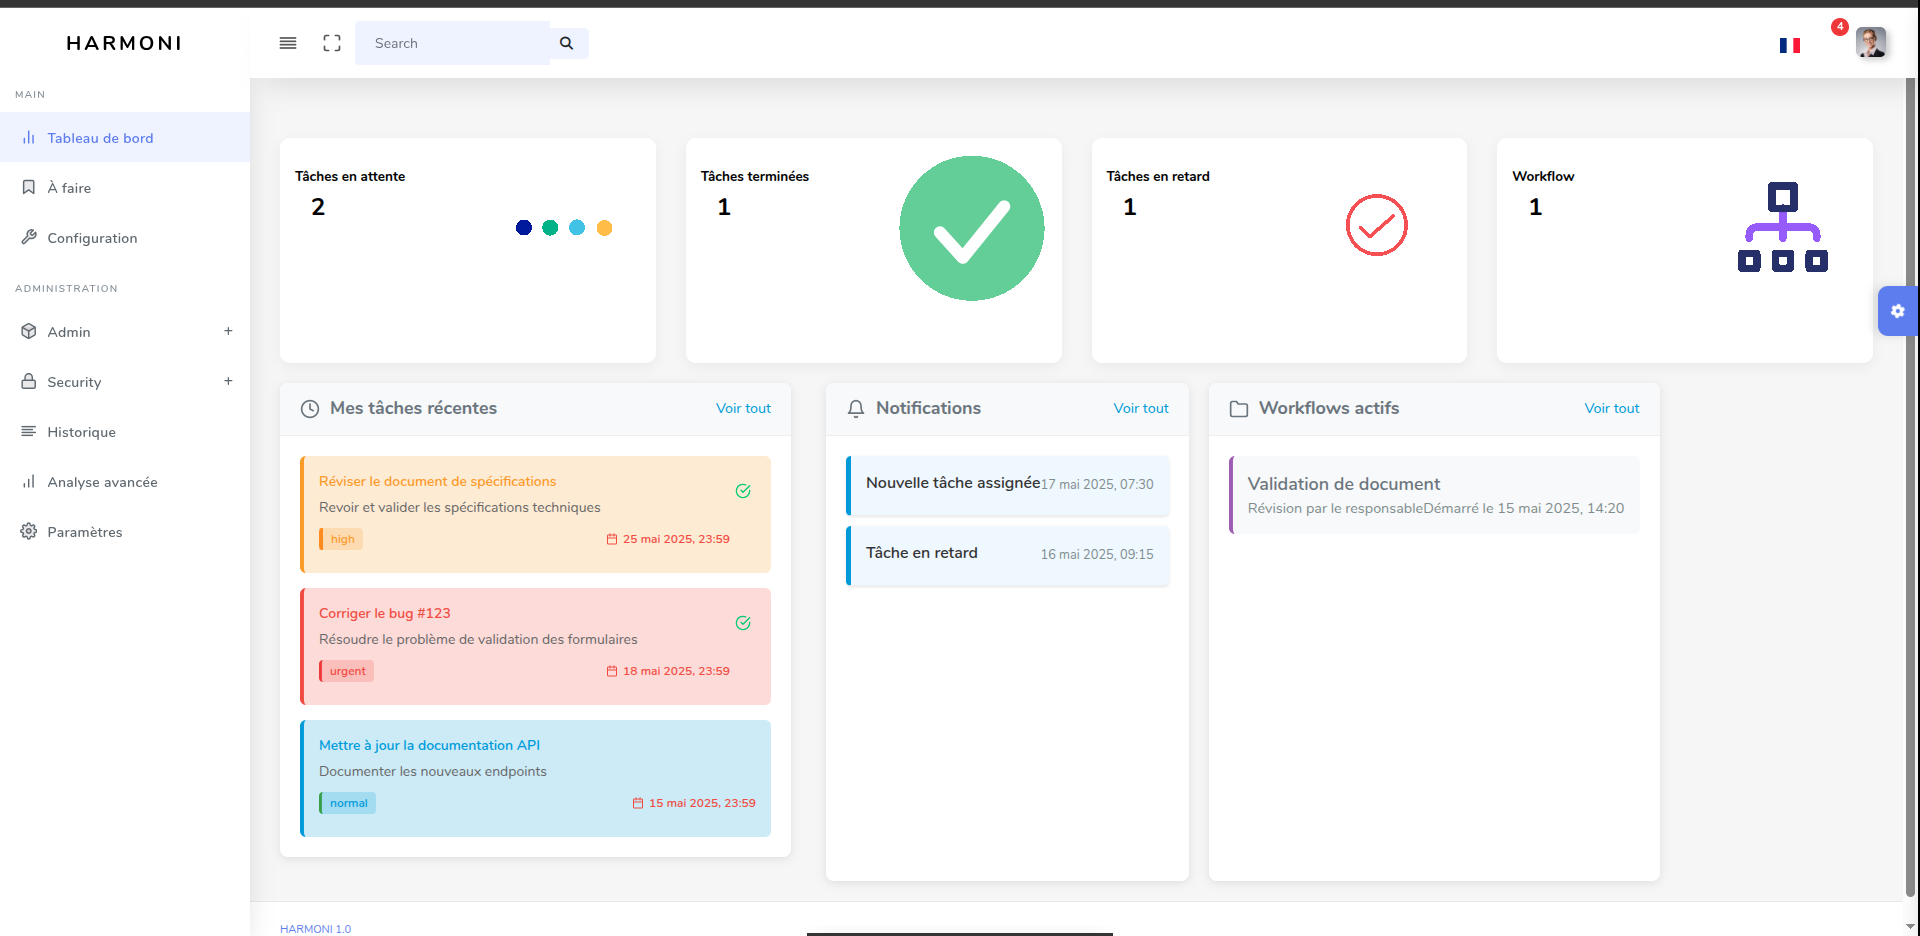
\includegraphics[width=0.9\textwidth]{Images/dashboard.png}
    \caption{Tableau de bord (Dashboard) — vue générale de Harmoni}
    \label{fig:dashboard}
\end{figure}

\paragraph{Description de la capture.}  
La figure~\ref{fig:dashboard} montre le tableau de bord principal : indicateurs-clés (nombre d'instances actives, taux d'échec, temps moyen de traitement), liste d'instances récentes, filtres globaux (par processus, par statut, par utilisateur) et accès rapides aux actions (nouveau modèle, déploiement, rapport). On y voit également des composants graphiques synthétiques (courbes temporelles, gauges).

\paragraph{Interprétation et validation.}  
Ce dashboard illustre la capacité de Harmoni à fournir une supervision centralisée en temps réel. Il valide le besoin de suivi opérationnel (monitoring) et facilite la prise de décision rapide par les gestionnaires de processus. Les KPI démontrent la conformité aux exigences non fonctionnelles en matière d’ergonomie et d’observabilité.

\section{Modélisation BPMN}

\begin{figure}[H]
    \centering
    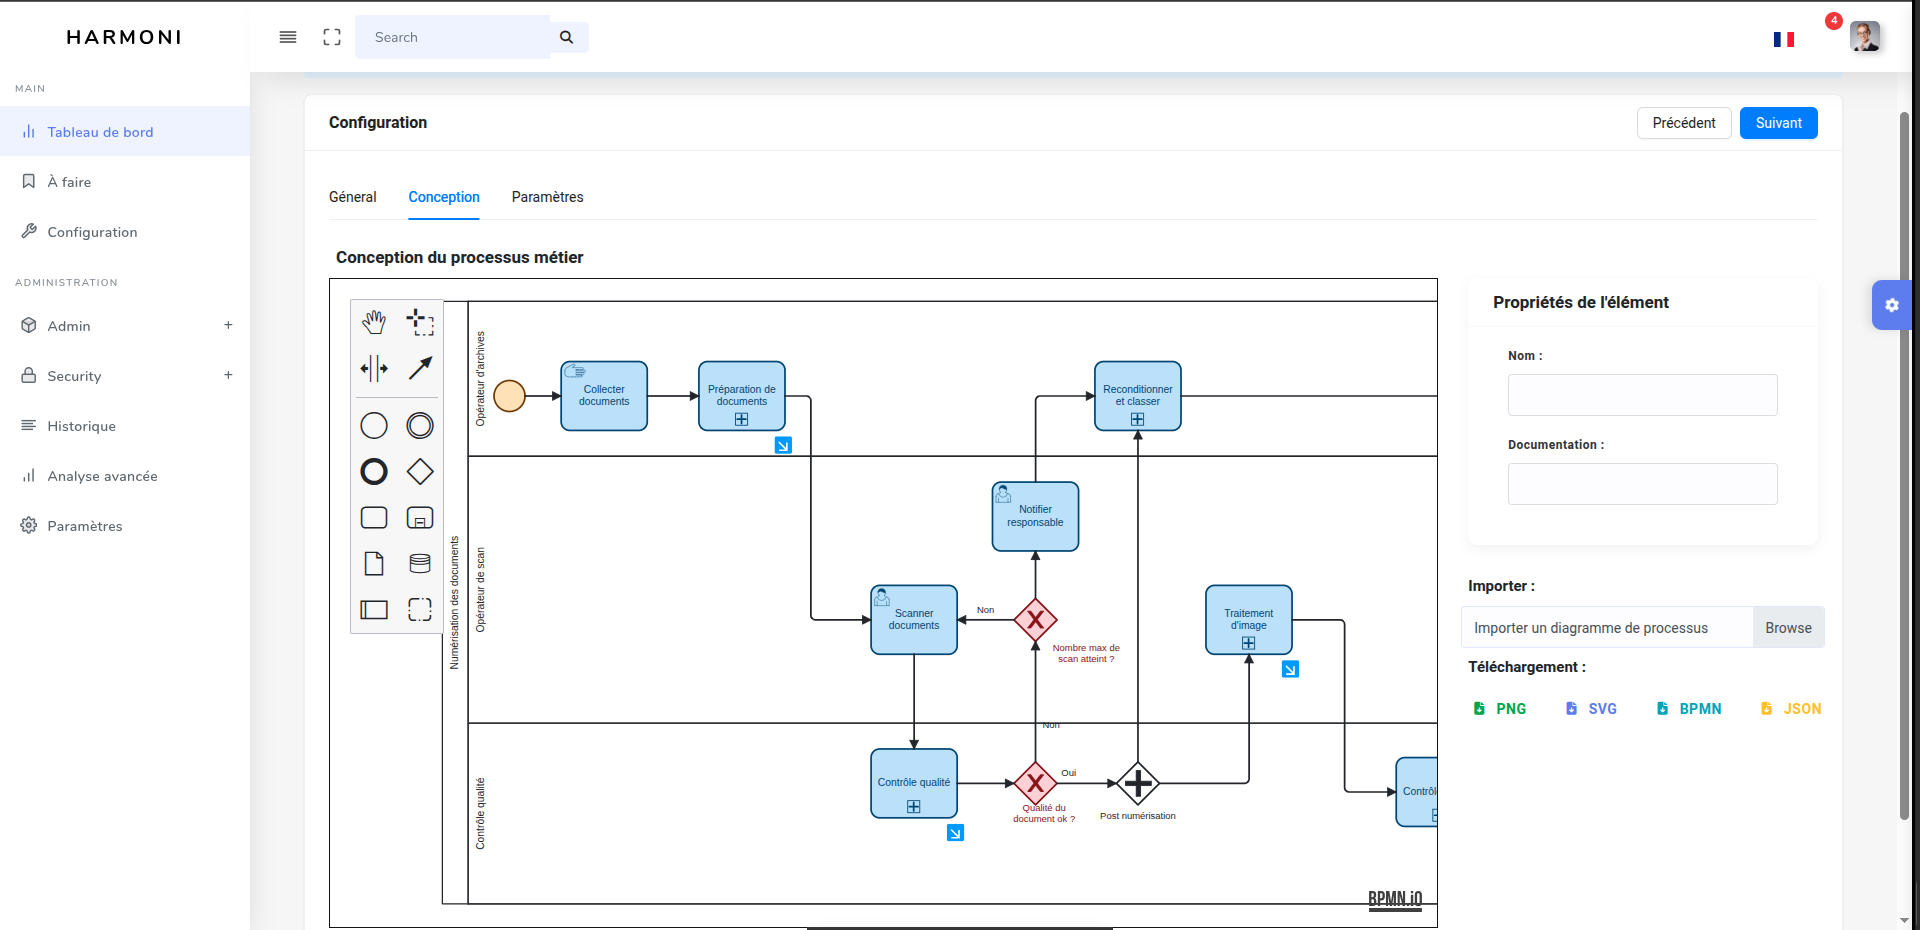
\includegraphics[width=0.9\textwidth]{Images/configuration.png}
    \caption{Éditeur BPMN — modélisation graphique}
    \label{fig:modelisation}
\end{figure}

\paragraph{Description de la capture.}  
La figure~\ref{fig:modelisation} montre l’éditeur intégré (canvas) avec la palette d’éléments BPMN (événements, tâches, passerelles), le panneau de propriétés contextuelles (configuration d’un élément sélectionné) et la barre d’outils (sauvegarde, validation, import/export BPMN XML).

\paragraph{Interprétation et validation.}  
Cette capture confirme que Harmoni permet la création visuelle des processus (glisser-déposer), l’édition des propriétés et la validation syntaxique BPMN. Elle valide le besoin fonctionnel de modélisation intuitive et l’interopérabilité via les formats BPMN standard (import/export).

\section{Configuration des tâches}

\begin{figure}[H]
    \centering
    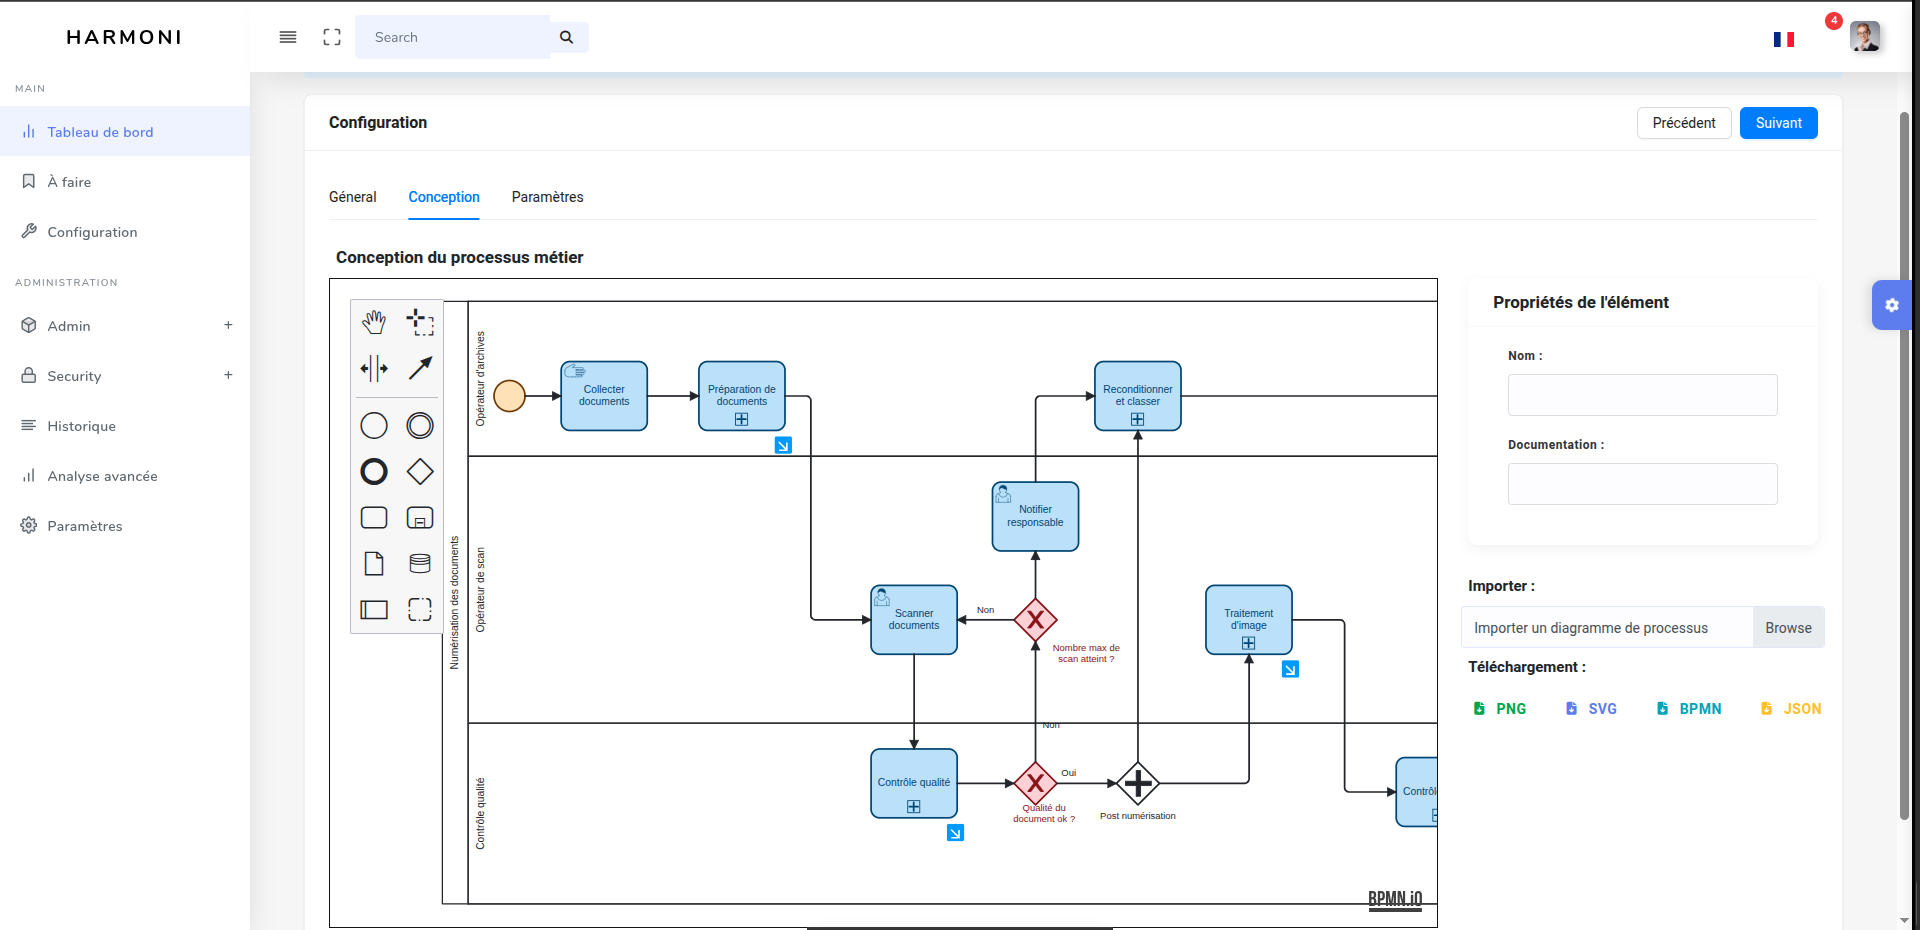
\includegraphics[width=0.9\textwidth]{Images/configuration.png}
    \caption{Configuration d’une tâche — affectation, règles et paramètres}
    \label{fig:configuration}
\end{figure}

\paragraph{Description de la capture.}  
La figure~\ref{fig:configuration} présente le panneau de configuration d’une tâche : affectation par utilisateur/groupe, SLA (délais), paramètres d’exécution (retries, timeout), mappage des variables et hooks de service (appel à un connecteur documentaire).

\paragraph{Interprétation et validation.}  
Cette vue montre comment les décisions de conception (backend Spring Boot + moteur BPMN) sont exposées côté frontend pour permettre une configuration fine des tâches. Elle valide la traçabilité des paramètres d’exécution et la compatibilité avec l’intégration documentaire (connecteurs Kairos).

\section{Kanban utilisateur}

\begin{figure}[H]
    \centering
    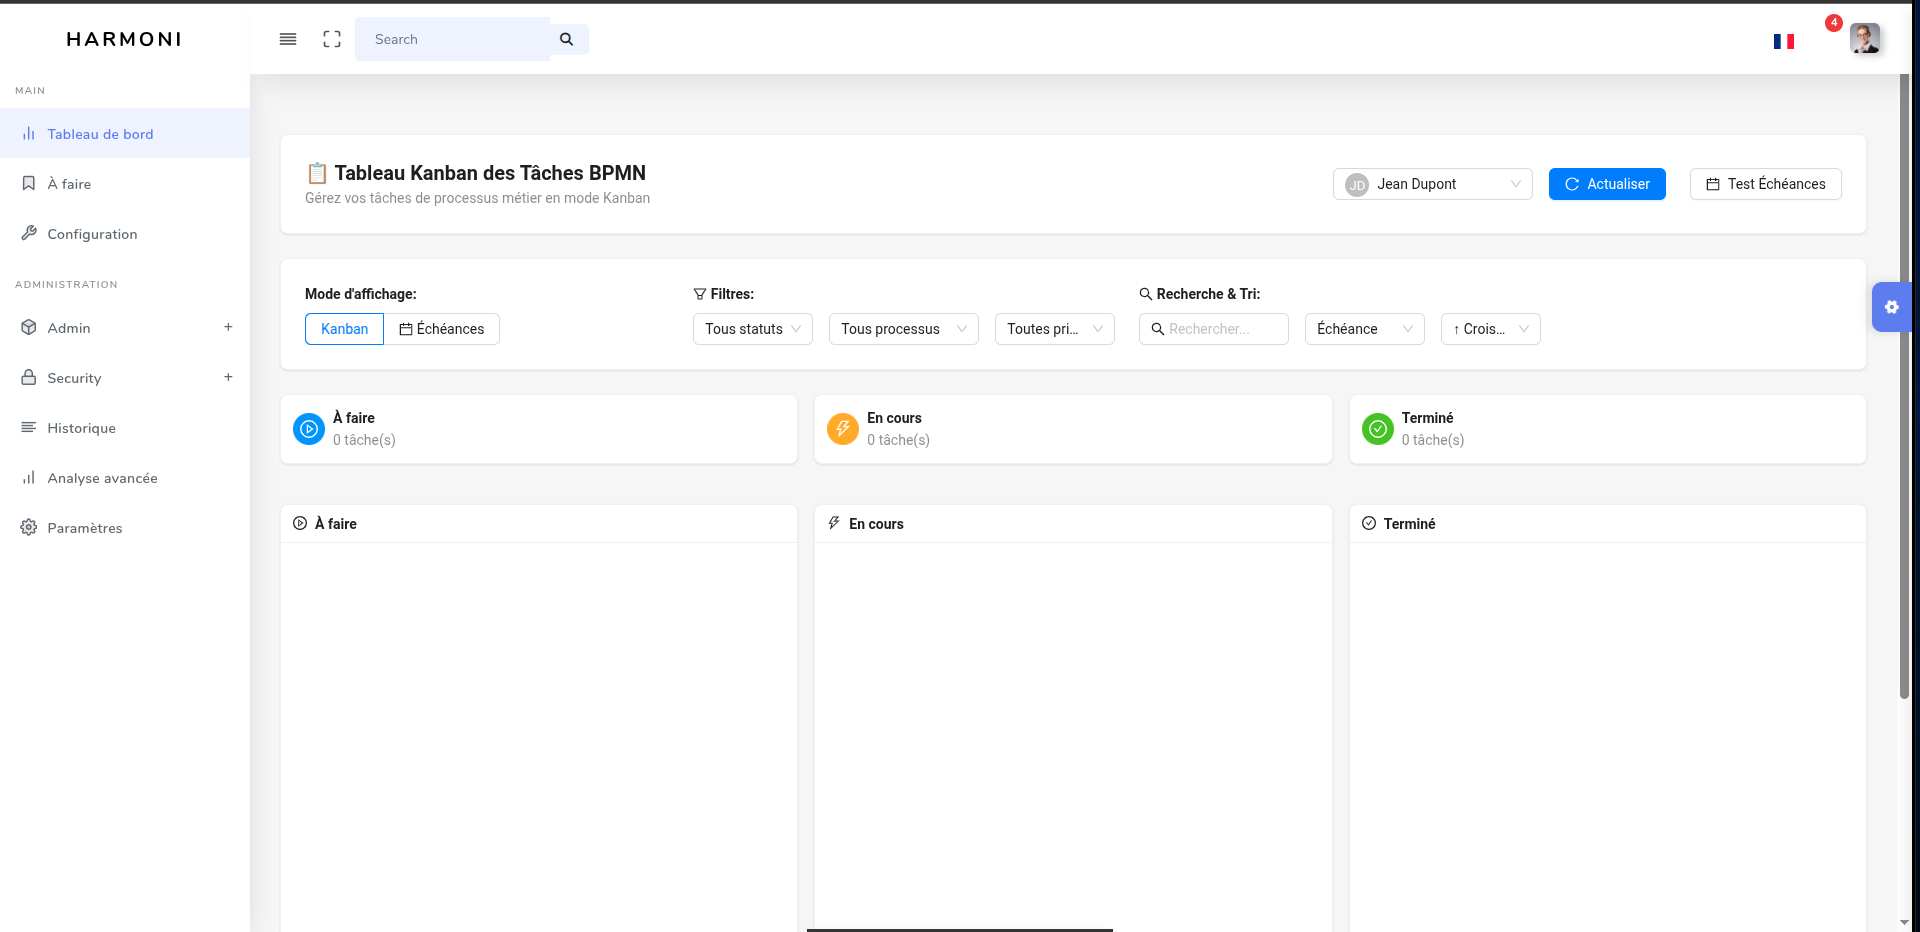
\includegraphics[width=0.9\textwidth]{Images/task.png}
    \caption{Tableau Kanban — gestion et priorisation des tâches par utilisateur}
    \label{fig:kanban}
\end{figure}

\paragraph{Description de la capture.}  
La figure~\ref{fig:kanban} illustre le tableau Kanban personnalisé : colonnes par statut (À faire, En cours, En attente, Terminé), cartes représentant les tâches/processus, actions rapides (assigner, commenter, déplacer), filtres et recherche.

\paragraph{Interprétation et validation.}  
Le Kanban traduit la capacité opérationnelle pour les utilisateurs finaux : gestion quotidienne des tâches, priorisation et collaboration. Il valide le besoin fonctionnel d’un tableau de bord utilisateur pratique et montre la synchronisation en temps réel entre le moteur d’exécution et l’interface.

\section{Notifications en temps réel}

\begin{figure}[H]
    \centering
    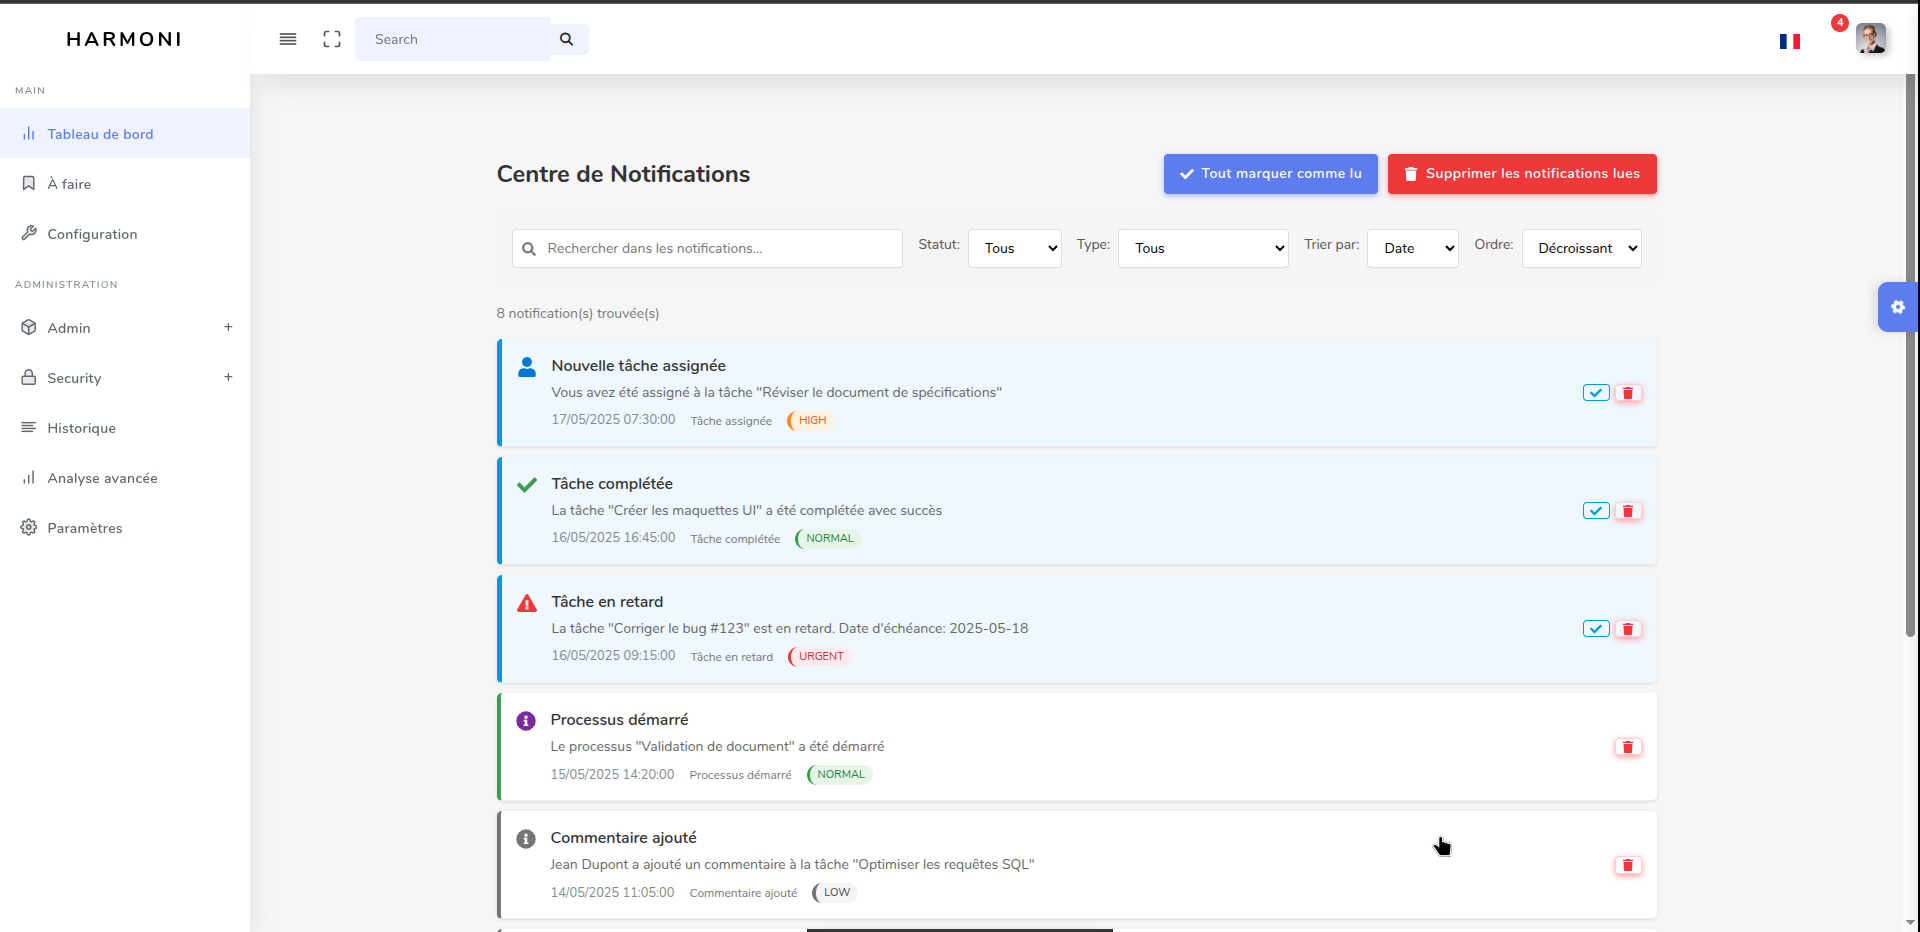
\includegraphics[width=0.9\textwidth]{Images/notification.png}
    \caption{Centre de notifications / alerte en temps réel}
    \label{fig:notification}
\end{figure}

\paragraph{Description de la capture.}  
La figure~\ref{fig:notification} présente l’interface de notifications : toasts en temps réel, historique des notifications, paramétrage des types d’alertes (échec d’instance, dépassement SLA, approbation requise) et liens directs vers l’instance concernée.

\paragraph{Interprétation et validation.}  
Les notifications démontrent la réactivité du système et la capacité à prévenir les acteurs des événements critiques. Elles répondent aux exigences métier d’alerte et de réactivité (SLA) et facilitent l’escalade opérationnelle.

\section{Historique et monitoring}

\begin{figure}[H]
    \centering
    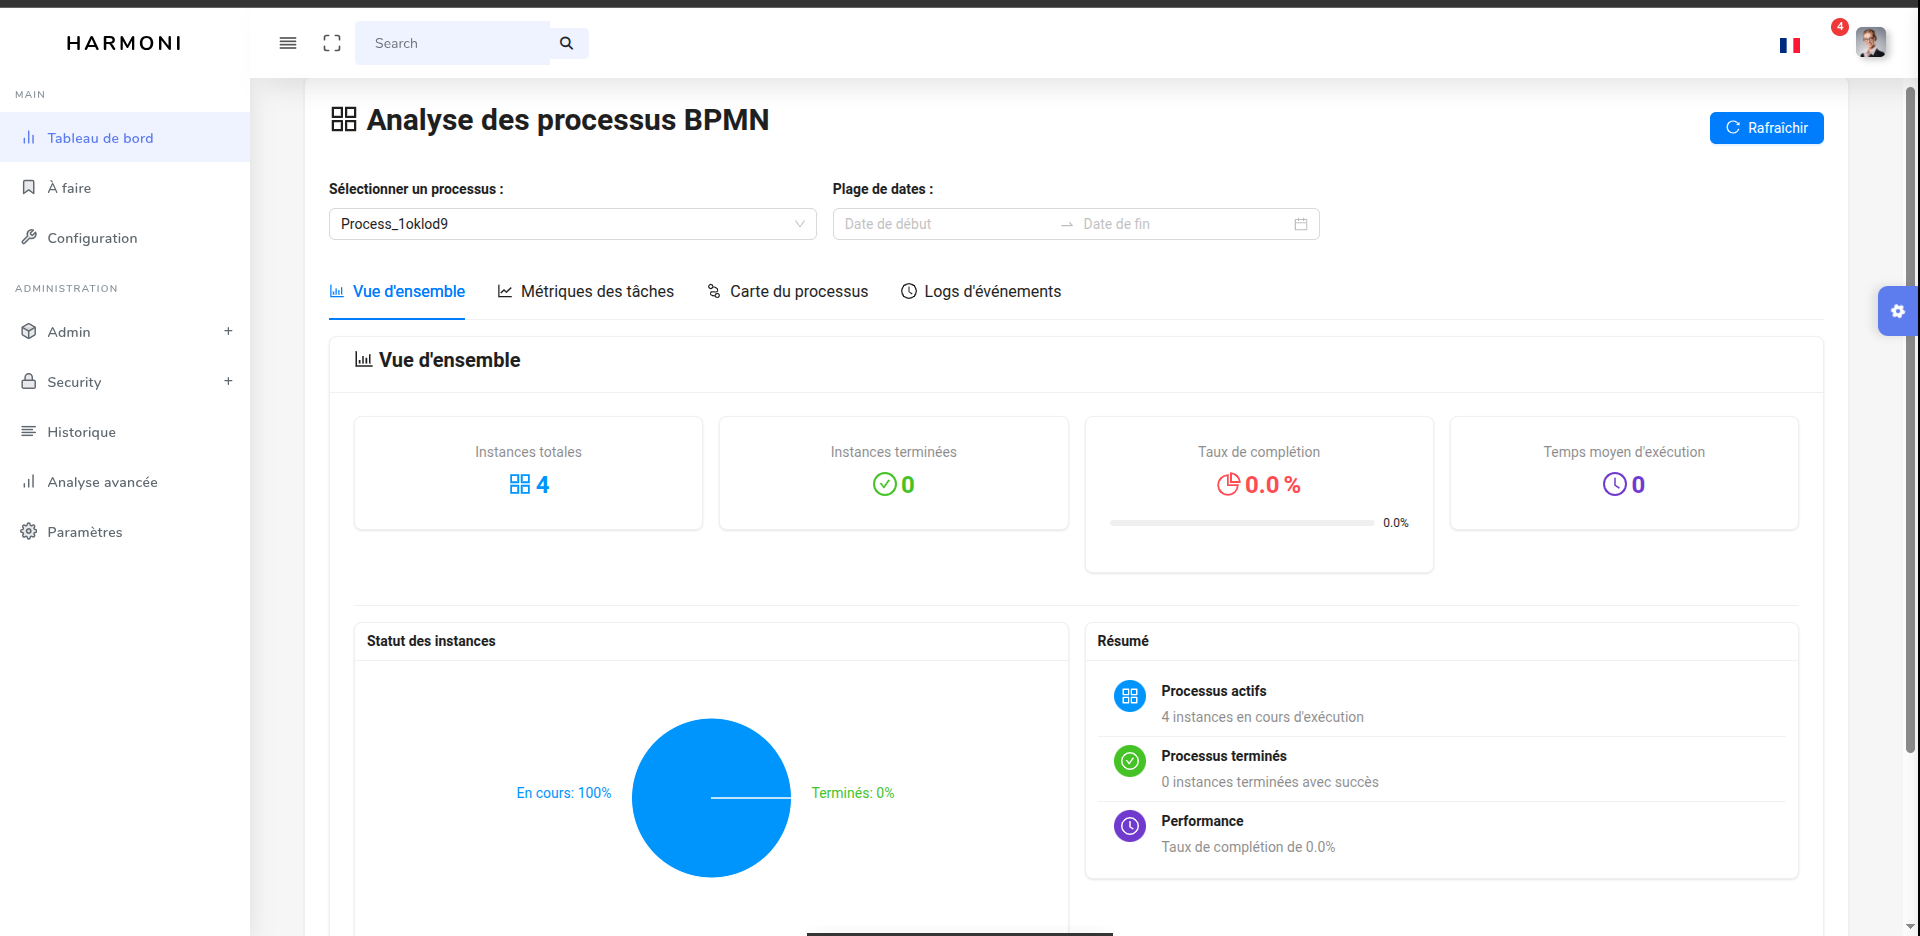
\includegraphics[width=0.9\textwidth]{Images/historique.png}
    \caption{Historique des exécutions et vue détaillée d’une instance}
    \label{fig:historique}
\end{figure}

\paragraph{Description de la capture.}  
La figure~\ref{fig:historique} montre la liste des instances (actives et terminées), leurs durées, événements marquants, journaux d’exécution et possibilité de relecture / export des logs pour audit.

\paragraph{Interprétation et validation.}  
Cet historique est essentiel pour la conformité et le debugging. Il valide les besoins non fonctionnels liés à la traçabilité, la gouvernance et la fiabilité. Les fonctionnalités d’export et d’archivage facilitent le reporting et les audits internes.

\section{Analyses BPMN avancées}

\begin{figure}[H]
    \centering
    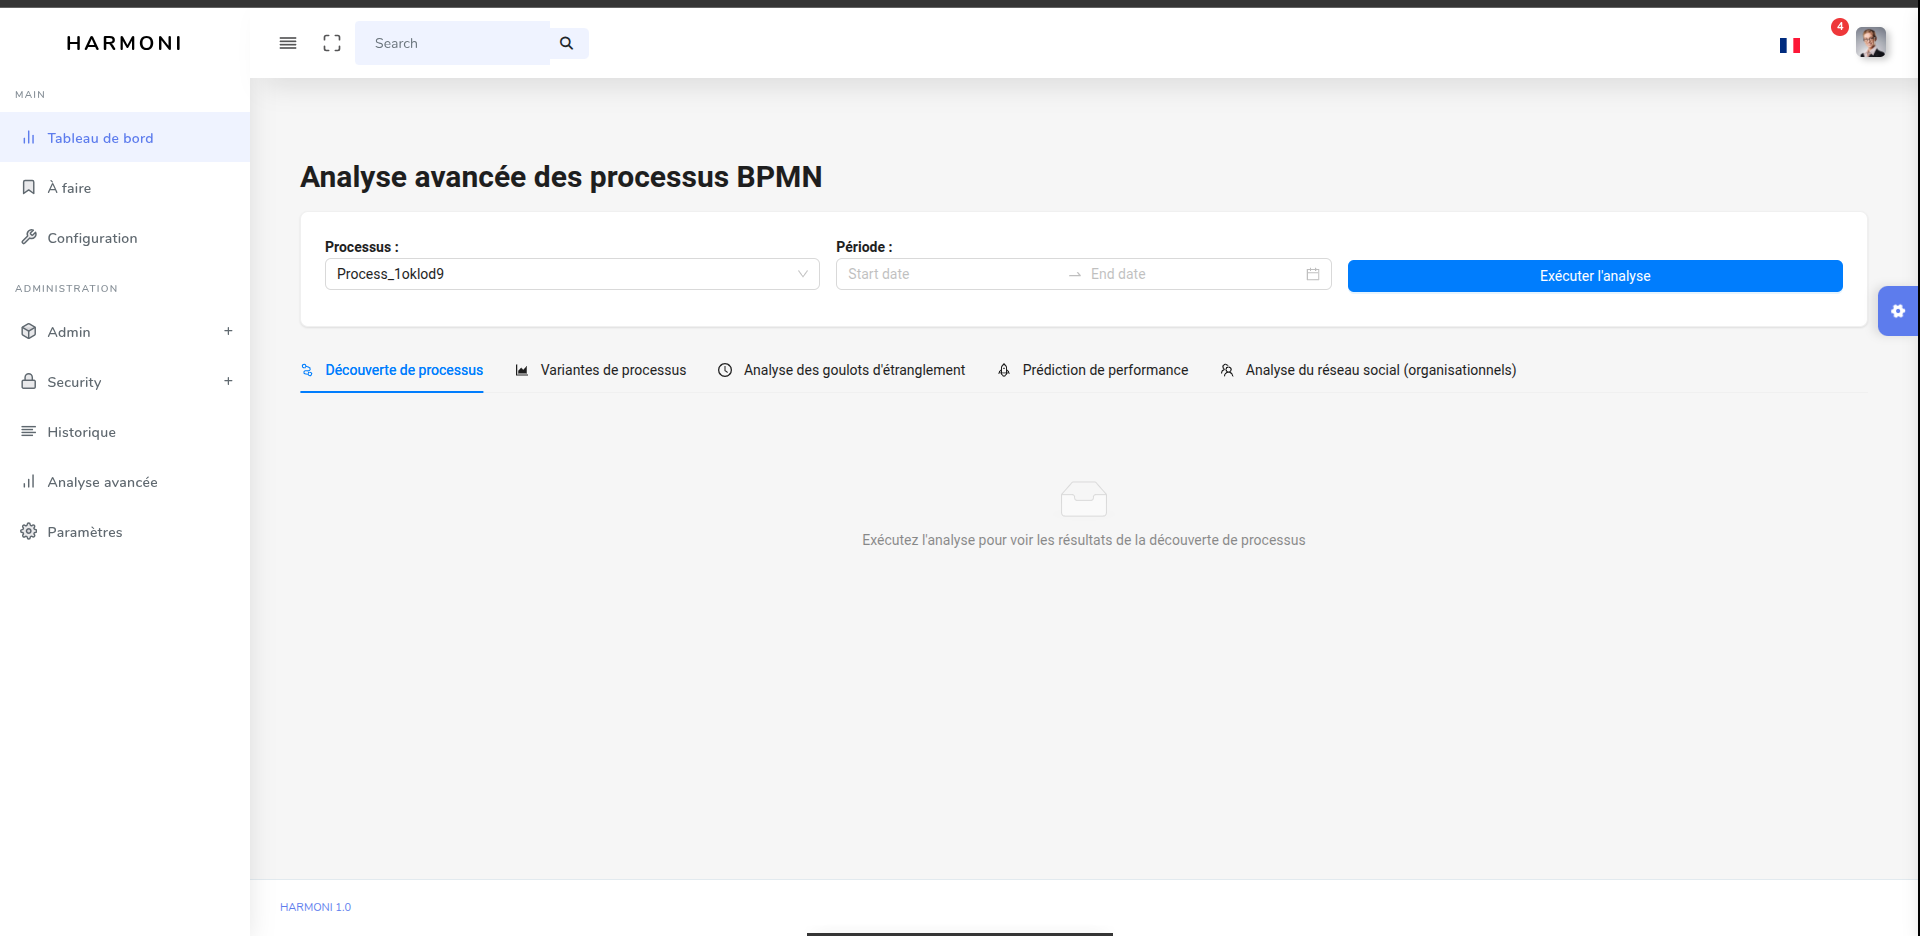
\includegraphics[width=0.9\textwidth]{Images/avancee.png}
    \caption{Module d’analyse — variantes, goulets, prédictions et réseau social organisationnel}
    \label{fig:analyse}
\end{figure}

\paragraph{Description de la capture.}  
La figure~\ref{fig:analyse} illustre l’interface analytique : visualisation des variantes de processus (heatmap / arbres de variantes), histogrammes des temps par activité (goulets d’étranglement), courbes de prédiction de fin d’instance, et graphe de réseau social montrant les interactions entre ressources.

\paragraph{Interprétation et validation.}  
Ces outils analytiques confirment l’apport scientifique et opérationnel de Harmoni :  
\begin{itemize}
    \item \textbf{Analyse des variantes} : identifie les chemins majoritaires et les divergences « as-is » vs modèle théorique ; utile pour prioriser les améliorations.
    \item \textbf{Détection des goulets} : mesure les temps d’attente / traitement et localise les points à optimiser.
    \item \textbf{Prédiction de performance} : fournit des estimations et alertes proactives pour respecter les SLA.
    \item \textbf{Réseau social} : met en évidence les acteurs clés et risques de centralisation des connaissances.
\end{itemize}
Ces outputs valident la valeur ajoutée analytique attendue par Kairos.

\section{Synthèse et recommandations pour les captures}

\paragraph{Synthèse.}  
Les captures présentées démontrent que Harmoni couvre le cycle complet : modéliser, configurer, exécuter, suivre, analyser. Elles valident les exigences fonctionnelles (modélisation, exécution, monitoring) et non fonctionnelles (sécurité, traçabilité, ergonomie).


\chapter*{CONCLUSION GÉNÉRALE}
\label{ch:conclusion}
% Bibliography temporarily disabled (no citations yet)
% \bibliographystyle{plain}
% \bibliography{bibli}
\end{document}
